% This is the Oregon State University LaTeX template. To the best of my
% knowledge, most of the work was done by those acknowledged in beavtex.cls.

%%
%% Preamble
%%
% \documentclass{<something>} must begin each LaTeX document
\documentclass[double,12pt]{beavtex}
  \renewcommand{\familydefault}{\sfdefault}
% Added by CII
\usepackage{graphicx,latexsym}
\usepackage{amsmath}
\usepackage{amssymb,amsthm}
\usepackage{longtable,booktabs,setspace}
\usepackage[hyphens]{url}
\usepackage[colorlinks = true,
			urlcolor = blue,
			linkcolor = black,
			citecolor = black,
			anchorcolor = black]{hyperref}
\usepackage{lmodern}
\usepackage{float}
\floatplacement{figure}{H}
% End of CII addition
\usepackage{rotating} % Package added to allow the rotation of figures and chart
                      % on a page, {sidewaysfigure} command
\usepackage{tablefootnote} % Packaged added to allow footnotes in the tabular
                           % environment, use \tablefootnote command

% This has to do with a default pandoc thing
% http://tex.stackexchange.com/a/258486/77699
\providecommand{\tightlist}{%
  \setlength{\itemsep}{0pt}\setlength{\parskip}{0pt}}

% Added by CII (Thanks, Hadley!)
% Use ref for internal links
\renewcommand{\hyperref}[2][???]{\autoref{#1}}
\def\chapterautorefname{Chapter}
\def\sectionautorefname{Section}
\def\subsectionautorefname{Subsection}
% End of CII addition

% Added by CII
\usepackage{caption}
\captionsetup{width=5in}
% End of CII addition

\title{Development and Application of Tools for Analysis of Clonal Population
Genetics} % {An Analysis of Something}
\author{Zhian N. Kamvar} % {Joseph A. Student}
\degree{Doctor of Philosophy} % {Master of Science}
\doctype{Dissertation}
\submitdate{December 6, 2016} % {January 1, 2013}
\commencementyear{2017} % {2013}

\department{Botany and Plant Pathology} % {Nuclear Engineering and Radiation Health Physics}

\depttype{Department} % {School}

\depthead{Head} % {Director}

\major{Plant Pathology} % {Radiation Health Physics}

\advisor{Niklaus J. Grünwald} % {Jane R. Professor}

\abstract{This is a \LaTeX template derived from the \beavtex template found on
overleaf
(\url{https://www.overleaf.com/latex/templates/oregon-state-university-thesis-and-dissertation/wnvzcdhqshxf})
and cloned using
\texttt{git\ clone\ https://git.overleaf.com/5973847rnpkdf} I have made
the following changes

\begin{itemize}
\tightlist
\item
  modified \texttt{beavtex.cls} from v1.1 to include support for
  verbatim font styles in R code
\item
  stripped the template of its original content to create a pandoc
  template
\item
  placed this into a bookdown (\url{https://bookdown.org/}) framework
\item
  added packages latexsym, amsmath amssymb,amsthm, longtable, booktabs,
  setspace, url, hyperref, lmodern, caption, and float
\end{itemize}

This is still a WIP, but it seems to work for the moment. Zhian N.
Kamvar 2016-08-25}
\acknowledgements{I would like to acknowledge\ldots{}Lorem ipsum dolor sit amet,
consectetur adipiscing elit. Maecenas vel eros sed mauris porttitor
semper nec a orci. Nullam vestibulum mi nec condimentum posuere.
Pellentesque eget diam id sapien aliquet ullamcorper. Pellentesque
blandit nec lectus ut mollis. Praesent in facilisis justo. Vestibulum
ante ipsum primis in faucibus orci luctus et ultrices posuere cubilia
Curae; Sed eget congue leo, sed consequat libero. In rutrum malesuada
nisi. Vestibulum ante ipsum primis in faucibus orci luctus et ultrices
posuere cubilia Curae; Morbi sollicitudin tortor ut sem facilisis
mollis.}


	\contributors{The following people contributed to this dissertation:

\subsubsection*{Chapter 2}\label{chapter-2}
\addcontentsline{toc}{subsubsection}{Chapter 2}

Javier F. Tabima assisted in writing the code and design, Niklaus J.
Grünwald assisted in design, and editing of the manuscript.

\subsubsection*{Chapter 3}\label{chapter-3}
\addcontentsline{toc}{subsubsection}{Chapter 3}

Zhian N. Kamvar, Meredeth M. Larsen, Alan M. Kanaskie, Everett M.
Hansen, and Niklaus J. Grünwald\ldots{}

\subsubsection*{Chapter 4}\label{chapter-4}
\addcontentsline{toc}{subsubsection}{Chapter 4}

Jonah C. Brooks assisted in writing and testing the code. Niklaus J.
Grünwald assisted in the design, coördination of the collaborative
effort, and editing the manuscript.

\subsubsection*{Chapter 5}\label{chapter-5}
\addcontentsline{toc}{subsubsection}{Chapter 5}

Niklaus J. Grünwald assisted in the design, and editing of the
manuscript.}


	\dedication{This is for my mother who paved the way.}




\begin{document}

\maketitle
\mainmatter


  \chapter{Introduction}\label{introduction}
  
  \begin{itemize}
  \tightlist
  \item
    Plant Pathogens
  
    \begin{itemize}
    \tightlist
    \item
      Evolution and Adaptation
    \item
      Understanding clonal population dynamics (\emph{Phytophthora} and
      \emph{Zymoseptoria} examples)
    \end{itemize}
  \item
    Tools for analysis
  
    \begin{itemize}
    \tightlist
    \item
      Tools for clonal populations always come after sexual populations
    \item
      We wrote our own tools
    \end{itemize}
  \item
    Goals of my work
  
    \begin{enumerate}
    \def\labelenumi{\arabic{enumi}.}
    \tightlist
    \item
      development of computational tools to characterize populations
    \item
      application of these tools to address empirical and theoretical
      questions
    \end{enumerate}
  \end{itemize}
  
  \section{Population genetics of clonal
  organisms}\label{population-genetics-of-clonal-organisms}
  
  \begin{itemize}
  \tightlist
  \item
    Population genetics is traditionally centered around HWE
  \item
    Clonal populations violate basic statistical inference
  
    \begin{itemize}
    \tightlist
    \item
      non-independent samples (clones)
    \item
      excess heterozygosity
    \item
      Meselson effect (Butlin 2000; Welch \& Meselson 2000, 2001; Balloux
      \emph{et al.} 2003)
    \end{itemize}
  \end{itemize}
  
  \section{\texorpdfstring{The Genus
  \emph{Phytophthora}}{The Genus Phytophthora}}\label{the-genus-phytophthora}
  
  The genus \emph{Phytophthora}, translating to ``plant destroyer'' in
  Greek, contains over 100 species (Kroon \emph{et al.} 2012), many of
  which have significant impact on US agriculture. \emph{P. sojae} is a
  major problem on soybean, causing \$1-2 billion in losses each year
  (Tyler 2007). \emph{P. ramorum} is changing the landscape of the North
  American West due to its wide host range (Grünwald \emph{et al.} 2008),
  which results in devastating losses for the US forestry and nursery
  industries. And \emph{P. infestans}, which was a root cause of over a
  million deaths during the Irish Potato Famine and continues to be a
  problem on tomato and potato crops, resulting in losses exceeding \$6
  billion, annually (Haas \emph{et al.} 2009). \emph{Phytophthora spp.}
  are water molds characterized by production of oospores and biflagellate
  zoospores that place them into the Stramenopiles (Baldauf 2003). They
  are most closely related to golden brown algae and quite diverged from
  fungi.
  
  \subsection{life cycle}\label{life-cycle}
  
  \subsection{Sex and mating types}\label{sex-and-mating-types}
  
  \subsection{\texorpdfstring{Heterothallic, clonal: \emph{P.
  ramorum}}{Heterothallic, clonal: P. ramorum}}\label{heterothallic-clonal-p.-ramorum}
  
  \begin{itemize}
  \tightlist
  \item
    Sudden Oak Death
  \item
    Population genetics in US nurseries (Goss \emph{et al.} 2009)
  \end{itemize}
  
  \subsection{\texorpdfstring{Homothallic, partially clonal: \emph{P.
  syringae}}{Homothallic, partially clonal: P. syringae}}\label{homothallic-partially-clonal-p.-syringae}
  
  \begin{itemize}
  \tightlist
  \item
    Abundant in OR Nurseries (found in foliar isolates) (Parke \emph{et
    al.} 2014)
  \item
    Genetic structure uncharacterized
  \end{itemize}
  
  \section{Tools for analysis of clonal population
  genetics}\label{tools-for-analysis-of-clonal-population-genetics}
  
  Recommendations have been made for analysis (Arnaud-Hanod \emph{et al.}
  2007)
  
  \begin{itemize}
  \tightlist
  \item
    MLG diversity
  \item
    Genotype Accumulation Curve
  \item
    \(P_{sex}\) and \(P_{gen}\)
  \end{itemize}
  
  \subsection{Index of Association}\label{index-of-association}
  
  \begin{itemize}
  \tightlist
  \item
    Standardized Version (Agapow \& Burt 2001)
  \item
    Previous Simulation Analyses (de Meeûs \& Balloux 2004)
  \item
    What's missing
  
    \begin{itemize}
    \tightlist
    \item
      Sympatric clonal lineages
    \item
      Analysis of significance testing
    \item
      HTS markers
    \end{itemize}
  \end{itemize}
  
  \subsection{Software Limitations}\label{software-limitations}
  
  Plethora of tools, most designed for sexual populations except:
  
  \begin{itemize}
  \tightlist
  \item
    GenClone
  \item
    GenoDive
  \end{itemize}
  
  Problems with file formatting, time, and reproducibility.
  
  \subsection{poppr}\label{poppr}
  
  \begin{itemize}
  \tightlist
  \item
    R
  \item
    poppr
  \end{itemize}
  
  \section{Applications of novel tools for analysis of partially-clonal
  populations}\label{applications-of-novel-tools-for-analysis-of-partially-clonal-populations}
  
  \begin{itemize}
  \tightlist
  \item
    Simulation analysis of \(\bar{r}_d\)
  \item
    SSR analysis of \emph{P. ramorum}
  \item
    GBS analysis of \emph{P. syringae}
  \end{itemize}
  
  \section{Conclusion}\label{conclusion}
  
  \begin{itemize}
  \tightlist
  \item
    Open Source Scientific Software Development of Poppr
  
    \begin{itemize}
    \tightlist
    \item
      Related tools
    \end{itemize}
  \item
    Simulation Analysis
  \item
    Pop gen info for two \emph{Phytophthoras}
  \item
    Major results of your work in 2-4 sentences \ldots{}
  \end{itemize}
  
  \chapter{\texorpdfstring{\emph{Poppr}: an R Package For Genetic Analysis
  of Populations With Clonal, Partially Clonal, and/or Sexual
  Reproduction}{Poppr: an R Package For Genetic Analysis of Populations With Clonal, Partially Clonal, and/or Sexual Reproduction}}\label{poppr-an-r-package-for-genetic-analysis-of-populations-with-clonal-partially-clonal-andor-sexual-reproduction}
  
  Zhian N. Kamvar, Javier F. Tabima, and Niklaus J. Grünwald
  
  \vspace*{\fill}
  
  \textbf{Published in PeerJ 2014-03-04}
  
  DOI: \href{https://dx.doi.org/10.7717/peerj.281}{10.7717/peerj.281}
  
  \newpage
  
  \section{Abstract}\label{abstract}
  
  Many microbial, fungal, or oomcyete populations violate assumptions for
  population genetic analysis because these populations are clonal,
  admixed, partially clonal, and/or sexual. Furthermore, few tools exist
  that are specifically designed for analyzing data from clonal
  populations, making analysis difficult and haphazard. We developed the R
  package poppr providing unique tools for analysis of data from admixed,
  clonal, mixed, and/or sexual populations. Currently, poppr can be used
  for dominant/codominant and haploid/diploid genetic data. Data can be
  imported from several formats including GenAlEx formatted text files and
  can be analyzed on a user-defined hierarchy that includes unlimited
  levels of subpopulation structure and clone censoring. New functions
  include calculation of Bruvo's distance for microsatellites,
  batch-analysis of the index of association with several indices of
  genotypic diversity, and graphing including dendrograms with bootstrap
  support and minimum spanning networks. While functions for genotypic
  diversity and clone censoring are specific for clonal populations,
  several functions found in poppr are also valuable to analysis of any
  populations. A manual with documentation and examples is provided. Poppr
  is open source and major releases are available on CRAN:
  \url{http://cran.r-project.org/package=poppr}. More supporting
  documentation and tutorials can be found under `resources' at:
  \url{http://grunwaldlab.cgrb.oregonstate.edu/}.
  
  \chapter{Spatial and Temporal Analysis of Populations of the Sudden Oak
  Death Pathogen in Oregon
  Forests}\label{spatial-and-temporal-analysis-of-populations-of-the-sudden-oak-death-pathogen-in-oregon-forests}
  
  Zhian N. Kamvar, Meredeth M. Larsen, Alan M. Kanaskie, Everett M.
  Hansen, and Niklaus J. Grünwald
  
  \vspace*{\fill}
  
  \textbf{Published in Phytopathology 2015-07}
  
  DOI:
  \href{http://dx.doi.org/10.1094/PHYTO-12-14-0350-FI}{10.1094/PHYTO-12-14-0350-FI}
  
  \newpage
  
  \section{Abstract}\label{abstract-1}
  
  Sudden oak death caused by the oomycete \emph{Phytophthora ramorum} was
  first discovered in California toward the end of the 20th century and
  subsequently emerged on tanoak forests in Oregon before its first
  detection in 2001 by aerial surveys. The Oregon Department of Forestry
  has since monitored the epidemic and sampled symptomatic tanoak trees
  from 2001 to the present. Populations sampled over this period were
  genotyped using microsatellites and studied to infer the population
  genetic history. To date, only the NA1 clonal lineage is established in
  this region, although three lineages exist on the North American west
  coast. The original introduction into the Joe Hall area eventually
  spread to several regions: mostly north but also east and southwest. A
  new introduction into Hunter Creek appears to correspond to a second
  introduction not clustering with the early introduction. Our data are
  best explained by both introductions originating from nursery
  populations in California or Oregon and resulting from two distinct
  introduction events. Continued vigilance and eradication of nursery
  populations of \emph{P. ramorum} are important to avoid further
  emergence and potential introduction of other clonal lineages.
  
  \section{Introduction}\label{introduction-1}
  
  Sudden oak death (SOD) emerged as a severe epidemic disease on coast
  live oak (\emph{Quercus agrifolia}) and tanoak (\emph{Notholithocarpus
  densiflorus}) in California in the mid 1990s and reemerged shortly
  thereafter on tanoak in Oregon in the early 2000s (Hansen et al. 2008;
  Rizzo et al. 2005; Grünwald et al. 2008a; Everhart et al. 2014). SOD is
  caused by \emph{Phytophthora ramorum} Werres, De Cock \& Man in't Veld,
  and is considered to be one of the top two oomycete pathogens based on
  its scientific and economic importance
  
  (Kamoun et al. 2014; Werres et al. 2001). The Oregon epidemic was first
  detected during aerial surveys in 2001 on tanoak but likely derived from
  initial introductions in the late 1990s. The Oregon Department of
  Forestry has since monitored the epidemic and sampled symptomatic
  tanoaks since 2001 (Hansen et al. 2008). Strains sampled from infected
  sites in forest or nursery environments have been genotyped in several
  labs using a range of microsatellite loci (Grünwald et al. 2009; Ivors
  et al. 2006; Prospero et al. 2004, 2007, 2009).
  
  \emph{P. ramorum} has emerged repeatedly around the world as 4 distinct
  clonal lineages found in North America (lineages NA1, NA2, and EU1) and
  Europe (EU1 and EU2) (Grünwald et al. 2012; Ivors et al. 2006; Van
  Poucke et al. 2012). The lineages have been named by the continent on
  which they first appeared, i.e.~North America (= NA) or Europe (= EU)
  and are numbered in order of discovery (Grünwald et al. 2009). The NA1
  clonal lineage was first discovered in California causing SOD on tanoak
  and coast live oak and is the one currently found in Curry County,
  Oregon, USA (Mascheretti et al. 2008). The EU1 and NA2 populations were
  discovered later in nursery environments and are currently only found in
  California, Oregon, Washington and British Columbia while the NA1 clone
  has been shipped with nursery plants from the West to the Southern and
  Southwestern US (Goss et al. 2011; Grünwald et al. 2012; Goss et al.
  2009; Ivors et al. 2006; Prospero et al. 2009; Mascheretti et al. 2008).
  The EU1 clonal lineage is the one first discovered in Europe, but in
  2007 the new EU2 lineage emerged in Northern Ireland and since migrated
  to Western Scotland (Werres et al. 2001; Van Poucke et al. 2012). EU1
  was first introduced to Europe and eventually migrated to the Pacific
  Northwest of North America (Goss et al. 2011).
  
  \emph{P. ramorum} populations sampled in Oregon forests to date belong
  exclusively to the NA1 clonal lineage (Hansen et al. 2008; Prospero et
  al. 2007). Given that NA2 and/or EU1 clones have been found in
  California, Oregon, Washington, and/or British Columbia in association
  with nursery plant movements, introduction of NA2 or EU1 from nursery
  environments to Curry County forests is a plausible scenario (Goss et
  al. 2011, 2009; Grünwald et al. 2012; Prospero et al. 2009, 2007). Our
  present work thus monitors populations and potential emergence of novel
  lineages in Oregon forests.
  
  Our main objectives here are to describe the spatial and temporal
  pattern of the populations and clonal dynamic of the SOD pathogen in
  Curry County in southwestern Oregon from 2001 to the present.
  Specifically, we asked (1) if novel lineages have been introduced into
  the forests in Curry County, (2) if multiple introductions occurred, and
  (3) whether introduction might have come from nursery populations. We
  sampled infected tanoaks between 2001-2014 and characterized populations
  using microsatellite analysis.
  
  \section{Materials and Methods}\label{materials-and-methods}
  
  \textbf{Location.} The SOD infested areas are located in the Siskiyou
  Mountains of Curry County in south western Oregon near the town of
  Brookings (42.0575\(^{\circ}\) N, 124.2864\(^{\circ}\) W) on the coast
  (Figure \ref{fig:ramorum1}) (Prospero et al. 2007). The Siskiyou
  mountains form part of the Klamath Mountain range (Franklin and Dyrness
  1988). The vegetation in SOD infested areas is a mosaic of different
  vegetation types including mixed-evergreen, redwood (\emph{Sequoia
  sempervirens}) and Douglas-fir (\emph{Pseudotsuga menziesii}) forests
  with tanoak as the dominant SOD host.
  
  \begin{figure}
  
  {\centering \includegraphics[width=0.8\linewidth]{figure/phytopathology/figure_1} 
  
  }
  
  \caption[Spatial distribution of the SOD epidemic and multilocus genotypes of
  \emph{Phytophthora ramorum} in Curry County, Oregon.]{Spatial distribution of the SOD epidemic and multilocus genotypes of
  \emph{Phytophthora ramorum} in Curry County, Oregon. The yellow crosses
  mark tanoak trees found positive for \emph{P. ramorum} during aerial
  surveys. A total of 70 multilocus genotypes have been identified between
  2001-2014 and are marked by color as shown in the legend. The
  abbreviations for regions shown in the map are explained in Table 1. The
  inset shows the placement of Curry county (red dot) in SW Oregon.}\label{fig:ramorum1}
  \end{figure}
  
  \textbf{Sampling.} Commencing in 2001, 2-4 aerial surveys per year were
  conducted over the tanoak range by the Oregon Department of Forestry and
  the USDA Forest Service in Curry County. The survey detects recently
  killed tanoaks based on the reddish-brown color of foliage (Hansen et
  al. 2008). All trees identified by aerial surveys were ground checked
  and geographically referenced using a hand-held GPS instrument (Garmin
  GPS 12XL or 60CX, Garmin International, Olathe, KS). Bark or foliage
  samples were collected for determination of \emph{P. ramorum} presence
  by culturing in the field and laboratory. Host plants within the area of
  the delimitation survey, generally 300 feet, were also inspected and
  sampled if they were symptomatic. Maps of distribution were prepared
  using ArcView GIS version 3.3 and ArcMap version 10.2 (Environmental
  Systems Research Institute, Redlands, CA).
  
  \textbf{Isolation, identification and DNA extraction.} Isolations were
  made from symptomatic plant tissue onto selective CARP agar (Difco corn
  meal agar, 10 ppm natamycin, 200pm NA-ampicillin, and 10 ppm rifampicin)
  (Prospero et al. 2007). Candidate \emph{Phytophthora} cultures were
  transferred onto corn meal agar with 30 ppm \(\beta\)-sitosterol.
  \emph{P. ramorum} identification was confirmed by microscopic inspection
  for presence of characteristic chlamydospores and deciduous sporangia
  (Werres et al. 2001). Genomic DNA was extracted using either the FastDNA
  SPIN kit (MP Biomedicals, LLC; 116540600) (Goss et al. 2009) or the
  cetyltrimethyl ammonium bromide (CTAB)-chloroform-isopropanol method
  (Winton and Hansen 2001). Table 1 provides an overview of strains
  collected by year and region following regions as shown in figure 1.
  
  \textbf{Genotyping, data validation, and harmonization.} Five
  microsatellite loci were utilized in this analysis: PrMS6, Pr9C3,
  PrMS39, PrMS45, and PrMS43 (Grünwald et al. 2009; Prospero et al. 2004,
  2007; Grünwald et al. 2008b). Genotyping (see specific protocols in
  supplementary text) of \emph{P. ramorum} strains collected 2001-2012
  occurred over several years and in several laboratories, with different
  protocols and sequencers. Consequently, a concerted effort was made to
  create a comprehensive dataset with identical allele calls. To detect
  errors, allele calls from all five genotyped loci were generated for a
  subsample of 40 isolates representing the most common multilocus
  genotypes from the culture collection, and then compared to data from
  participating laboratories. Three of the five loci, PrMS6, Pr9C3, and
  PrMS39 had identical allele calls between laboratories for the
  subsampled isolates. The remaining two loci, PrMS45 and PrMS43, had
  allele calls that differed by a single bp between laboratories. Data
  from PrMS45 and PrMS43 were therefore corrected to allow consistent
  comparisons of allele calls. Given the varied nature of the genotyping
  data described above genotyping of \emph{P. ramorum} strains consists of
  two datasets including either 5 loci (2001-14) or a newly developed,
  multiplexed method including 14 loci (samples 2013-14) (Table 2).
  Details on both genotyping methods can be found in the supplementary
  text and figure S1.
  
  \textbf{Nursery populations.} To determine if forest populations cluster
  with different nursery populations from Oregon or California, we used
  previously published data from our work to determine relationships among
  nursery and Curry County forest populations (Goss et al. 2011, 2009;
  Grünwald et al. 2009; Prospero et al. 2009, 2007).
  
  \textbf{Data analysis.} All individuals genotyped for this effort
  belonged to the NA1 clonal lineage (Grünwald et al. 2009). Thus, all
  analyses presented here focused on describing the clonal dynamic using
  model-free approaches that avoid violation of population genetic theory.
  Samples were grouped into different multilocus genotypes (MLGs) defined
  by the unique combination of alleles across all observed loci from the
  consensus five SSR loci genotyped across all years. For identification
  purposes, unique MLGs were then assigned an arbitrary number from 1 to
  the total number of observed MLGs. Population genetic analysis was
  conducted using the computer and statistical language R (R Core team
  2014) using various packages as well as R functions written specifically
  for this project (see github link below). Graphs and figures were
  created using the R packages \emph{ggplot2, ape, igraph, ggmap,} and
  \emph{poppr} (Wickham 2009; Csardi and Nepusz 2006; Paradis et al. 2004;
  Kahle and Wickham 2013; Kamvar et al. 2014). Within-locus allelic
  diversity was analyzed across and within years and regions using the
  function \texttt{locus\textbackslash{}\_table} from the R package
  \emph{poppr} (Table S1)(Kamvar et al. 2014). To address the temporal and
  spatial aspects of the data, populations were analyzed both by year
  isolated and watershed region (Table 1; Fig. 1). Watershed regions were
  drawn with ArcMap version 10.2 (Environmental Systems Research
  Institute, Redlands, CA). The regions represent drainages or portions of
  drainages in which infected trees were discovered as the disease
  progressed over time. In most cases, ridgelines dividing drainages
  formed the boundary of a region. These regions were saved as shapefiles
  and imported into R with rgdal (Bivand et al. 2014).
  
  Genotypic diversity was analyzed within and across years and
  populations, with the Shannon-Wiener index (\emph{H}) and the Stoddard
  and Taylor's index (\emph{G}), (Shannon and Weaver 1949; Stoddart and
  Taylor 1988). Both \emph{G} and \emph{H} measure genotypic diversity,
  combining richness and evenness. If all genotypes are equally abundant,
  then the value of \emph{G} will be the number of MLGs and the value of
  \emph{H} will be the natural log of the number of MLGs. Both \emph{G}
  and \emph{H} are used as they weigh more or less abundant MLGs more
  heavily, respectively (Grünwald et al. 2003). Evenness was calculated as
  \emph{E\textsubscript{5}}, which is an estimator of evenness that
  utilizes both \emph{H} and \emph{G} that gives a ratio of the number of
  abundant genotypes to rare genotypes (Grünwald et al. 2003; Pielou 1975;
  Ludwig 1988). These were calculated with the R packages \emph{poppr} and
  \emph{vegan} (Oksanen et al. 2013; Kamvar et al. 2014). Confidence
  intervals were calculated using the R package \emph{boot} with 9,999
  bootstrap resamplings (Canty and Ripley 2014). Richness, or the expected
  number of MLGs (\emph{eMLG}), was calculated using rarefaction from the
  R packages \emph{poppr} and \emph{vegan} (Hurlbert 1971; Heck et al.
  1975). Some statistics (AMOVA, genotypic diversity, index of
  association, allelic diversity, and Nei's distance) were also performed
  on clone-censored data where each MLG was represented once per
  population hierarchy.
  
  Because the analysis of genotypic diversity, richness and evenness is
  agnostic to specific alleles within MLGs, assessment of genetic
  relatedness between MLGs was performed using the function bruvo.dist
  using \emph{poppr}, which calculates Bruvo's genetic distance, utilizing
  a stepwise mutation model for microsatellite loci (Bruvo et al. 2004;
  Kamvar et al. 2014). This distance thus gives a more fine-scale picture
  of relationships between individuals than band-sharing models. These
  relationships were visualized with minimum spanning networks generated
  using the R packages \emph{igraph} and \emph{poppr} (Csardi and Nepusz
  2006; Kamvar et al. 2014).
  
  If the epidemic had a single origin, a correlation between genetic and
  geographic distance would be expected as populations acquire mutations
  over time and clonally diverge regardless of rates of spread. Divergence
  is affected by rates and distance of spread where long-distance
  dispersal or low rates of mutation would lead to less divergence and
  thus lower correlations between genetic and geographic distances. This
  was tested by performing Mantel tests across all hierarchical levels in
  the data set utilizing the function \texttt{mantel.randtest} in the R
  package \emph{ade4} between Bruvo's distance as described above and
  Euclidean distances between geographic coordinates (Mantel 1967; Dray
  and Dufour 2007). \emph{P}-values were calculated using 99,999 bootstrap
  replicates.
  
  As the eradication efforts destroy the immediate habitat in an infected
  area, one question that we wanted to address was whether or not
  genotypes were clustering to specific regions or if they were evenly
  spread throughout Curry County (Prospero et al. 2007). This was tested
  using three methods: bootstrap analysis of Nei's genetic distance,
  Analysis of MOlecular VAriance (AMOVA), and Discriminant Analysis of
  Principal Components (DAPC) in the R packages \emph{poppr}, \emph{ade4},
  and \emph{adegenet} (Jombart et al. 2010; Excoffier et al. 1992; Kamvar
  et al. 2014). The bootstrap analysis utilized 10,000 bootstrap
  replicates treating loci as independent units with the function aboot in
  \emph{poppr} and was visualized as an unrooted neighbor-joining tree in
  figtree v. 1.4.2 (Figure 3). AMOVA utilizes a distance matrix between
  genotypes for which hierarchical partitions are defined and attempts to
  analyze the variation within samples, between samples, between
  subpopulations within populations and finally between populations. In
  this case, we used both the hierarchies of samples within years within
  regions and samples within regions within years. DAPC is a multivariate,
  model-free approach to clustering based on prior population information
  (Jombart et al. 2010). This allows us to analyze the population
  structure by assessing how well samples can be reassigned into
  previously defined populations. Both DAPC and AMOVA were run with and
  without Hunter Creek and Pistol River South Fork due to isolated
  genotypes and small sample size, respectively. For the DAPC analysis,
  these removed populations had their origins predicted from the DAPC
  object using the function predict.dapc in the R package \emph{adegenet}
  (Jombart et al. 2010).
  
  Since DAPC is sensitive to the number of principal components used in
  analysis, the function xvalDapc from the R package \emph{adegenet} was
  used to select the correct number of principal components with 1,000
  replicates using a training set of 90\% of the data. The number of
  principal components was chosen based on the criteria that it had to
  produce the highest average percent of successful reassignment and
  lowest root mean squared error (Jombart et al. 2010). Significant
  deviations from random population structure was tested in AMOVA
  utilizing the function randtest from the R package \emph{ade4} with
  9,999 bootstrap replicates (Dray and Dufour 2007).
  
  All data and R scripts to reproduce the analyses shown here are
  deposited publicly on github
  (\url{https://github.com/grunwaldlab/Sudden_Oak_Death_in_Oregon_Forests})
  and citable (DOI: 10.5281/zenodo.13007).
  
  \section{Results}\label{results}
  
  \textbf{Demographic pattern and genetic diversity.} The epidemic has
  expanded over time from the initial focus in Joe Hall Creek NE of
  Brookings, Oregon mostly north (first to N Fork Chetco High) and
  northwest (Coast, Pistol River South Fork), but also east (Chetco Main
  and Winchuck) (Fig. 1; Table 1). To date a total of 70 multilocus
  genotypes have been found in forest populations (Table 1). MLG 22 is
  most abundant and the only MLG detected across the whole period
  (although it was not sampled in every year) (Fig. 2). MLG 59, the second
  most abundant MLG, was only detected in 2011 and has a high frequency
  due to the sampling design applied: all 2011 strains were sampled in one
  concentrated area in the northwestern sampling range geographically
  distant from any other location (Fig. 1). Given that sampling strategies
  for some years were not comprehensive, samples from some years have to
  be interpreted with caution (e.g., 2005-6, 2010-11). Samples from 2013
  and 2014 are sampled from all regions and can be considered more
  representative.
  
  Allelic and genotype diversity within loci revealed that PrMS43 had, on
  average, the highest number of alleles (n = 18). All other loci had 5 or
  fewer alleles with a moderate to high amount of diversity (Table S2).
  Nevertheless, the genotype accumulation curve showed a slight plateau,
  indicating that we have enough power in our data to describe a
  significant number of MLGs (Fig. S2). Genotypic diversity (\emph{H} =
  2.98, \emph{G} = 8.64), evenness (\emph{E\textsubscript{5}} = 0.41), and
  richness (\emph{eMLG} = 7) were low as expected for a clonal population
  slowly accumulating mutations over space and time (Table S3). A pattern
  of increasing diversity across years (with number of MLGs not fewer than
  10) was also observed (Table S3). The minimum spanning network showed
  that MLGs 17, 22, and 28 clustered in the center of the network and had
  the highest number of connections to other genotypes in the forest
  populations (Fig. 3). Most genotypes were connected to their immediate
  neighbors by a genetic distance of 0.05 or the equivalent of one
  mutational step across 5 diploid loci.
  
  \textbf{Spatial Correlation.} A Mantel test revealed significant
  correlations of genetic distance and geographic distance for most
  samples collected after 2003 (Table 3). When partitioned by year, this
  correlation appears to increase and become more pronounced with the
  progression of the epidemic. When partitioned by region, those that are
  closer to the origin of the epidemic (Joe Hall Creek and N Fork Chetco
  River) show significant correlation. When the overall mantel test was
  run without Hunter Creek, the correlation coefficient was reduced
  (0.175), but was still significant (\emph{p} = 0.0001).
  
  \textbf{Population differentiation.} Cluster analysis of populations
  with respect to year using Nei's genetic distance showed no significant
  (\textgreater70\%) bootstrap support for any clades, but does show that
  these tend to cluster by region as opposed to year (Fig. S3). AMOVA
  analysis revealed significant population structure between regions on
  both clone-corrected (with respect to hierarchy) and uncorrected data
  sets (Table 4). Significant structure was only found between years
  within regions on the uncorrected data set. Both patterns were observed
  without Hunter Creek and Pistol River South Fork isolates. DAPC
  clustering showed that the first discriminant component separated Hunter
  Creek from all other regions and the second discriminant component shows
  a gradient from Joe Hall Creek to the coast (Fig. 4). This distinction
  was reflected in the percent of correct posterior assignment of isolates
  to their original populations. Over the whole data set there was an
  81.5\% assignment-success rate. Hunter Creek received 100\% successful
  reassignment. Joe Hall Creek, Winchuck, and Coast all had
  \textgreater85\% successful reassignment whereas Chetco Main, North Fork
  of the Chetco, and Pistol River South Fork all had \textless{}69\%
  successful reassignment (Fig. S4). The isolation of the Hunter Creek
  isolates in the DAPC analysis was found to be mainly driven by allele
  493 at locus PrMS43 (Fig. S5). The only other population to share this
  allele was Joe Hall Creek where it was present in a total of 4 isolates,
  and only isolates found in the coastal region or North Fork Chetco
  contained the allele 489, which is one mutational step away in a
  stepwise mutation model of a tetranucleotide repeat locus. When DAPC was
  run without Hunter Creek and Pistol River South Fork data, percent
  successful reassignment for all regions did not change significantly.
  Prediction of sources for the Hunter Creek data revealed that over 98\%
  of the genotypes were assigned to the Coast with a 99\% probability.
  
  \textbf{Clustering of forest with nursery populations.} We used
  previously published data to determine if nursery populations in
  California or Oregon could have been source populations for the Oregon
  forest epidemic (Goss et al. 2011, 2009; Grünwald et al. 2009; Prospero
  et al. 2009, 2007). Nursery data included 40 MLGs across 216 samples of
  NA1 clones. Of these 40, 12 MLGs matched the forest sample and 28 MLGs
  were unique to the nurseries. The only region that did not contain
  genotypes that matched those found in nurseries was Pistol River South
  Fork. When considering those 12 genotypes that were present in both data
  sets, with the exception of Joe Hall Creek, all genotypes were first
  isolated from nurseries before discovery in the forest. At the most
  variable locus, PrMS43, both nursery populations had the allele 281 at
  frequencies of 4.5\% and 4.9\% for CA and OR, respectively. This allele
  was not observed in the forest population. Both populations contained
  allele 489 at \textgreater10\% frequency and the CA nursery population
  contained allele 493 at a frequency of 1.4\%.
  
  When nursery genotypes were added to the minimum spanning network, MLGs
  found at Hunter Creek, previously isolated in the network, connected by
  only a single MLG from the coast, gained more connections to nursery
  MLGs. Clustering with Nei's distance revealed the Nursery isolates from
  CA consistently clustering closest with Hunter Creek isolates in both
  clone-corrected and uncorrected data sets (Fig. 5). DAPC clustering
  revealed a decrease in overall assignment-success rate at 78\%. The
  nursery isolates received 74\% and 83\% assignment success for CA and OR
  nurseries, respectively.
  
  The assignment successes for the regions before or after inclusion of
  nursery data changed less than 5\% for all regions except for the coast,
  which saw a decrease of 17.6\% when nursery populations were included
  (Fig. S4). Prediction of sources for nursery genotypes against the
  forest data revealed that 48\% of these nursery isolates were predicted
  to share membership with the coast at \(\geq\) 95\% probability (Fig.
  S6, S7). A total of 3.2\% of the isolates were predicted to share
  membership with Hunter Creek at \(\geq\) 99.9\% membership probability.
  Furthermore, 21.75\% of the nursery data could not be assigned to any of
  the forest populations at \textgreater 60\% probability.
  
  Since 3.2\% of the nursery isolates had a very strong signal for Hunter
  Creek, we predicted sources for Hunter Creek isolates when considering
  nursery isolates. This approach determines if Hunter Creek isolates
  cluster more readily with nursery or coast populations. Indeed, 92\% of
  the Hunter Creek isolates were predicted to share membership with
  California nurseries at \(\geq\) 99\% membership probability (Fig. S8).
  No Hunter Creek isolate was predicted to share membership with a forest
  population at \textgreater0.45\% membership probability.
  
  \section{Discussion}\label{discussion}
  
  To date populations monitored from 2001-14 show presence of only the NA1
  clonal lineage observed previously (Prospero et al. 2007, 2009). The
  fact that individuals belonging to the EU1 and NA2 clonal lineages have
  not been found in Oregon forests, despite their presence on the west
  coast from British Columbia to California is welcome news (Goss et al.
  2009, 2011; Grünwald et al. 2012). The lack of EU1 or NA2 isolates
  provides evidence that monitoring for \emph{P. ramorum} in nurseries by
  federal and state agencies is helping avoid emergence of new clones in
  Oregon's Forests.
  
  Our analysis provides support for a most parsimonious scenario of two
  introductions into Curry county from nurseries: one initial introduction
  into Curry County sometime before detection of the first infected
  tanoaks in 2001 from California (or less likely Oregon) nurseries
  followed by a second introduction into the Hunter Creek area again from
  nurseries. The relative position of the nursery populations in the
  minimum spanning network and DAPC scatter plot (Fig. 3, 4) suggest that
  the introductions from nurseries were rare, though more even sampling
  and migration models could disprove this hypothesis. Since 2001, the
  epidemic has spread clonally throughout Southwestern Curry County mostly
  north, but also west, towards the coast, and southeast. This clonal
  spread of the pathogen from the Joe Hall area is supported partially by
  Mantel tests showing significant levels of isolation by distance in
  years following 2002 (Table 3) along with significant AMOVA results
  across regions (Table 4). The populations sampled in 2011 in Hunter
  Creek (Cape Sebastian) appear to have originated from a new source and
  cluster into a distinct group based on DAPC (Fig. 4). Based on the
  minimum spanning network, this population would appear isolated in the
  epidemic if it were not for MLG 32, which is connected with MLG 33
  (found on the coast in 2010) by one mutational step at locus PrMS43.
  This, in turn, is connected with the other MLGs from Hunter Creek by one
  mutational step at locus PrMS39. When considering clustering via Bruvo's
  distance in combination with data from nursery populations, however,
  these genotypes from Hunter Creek appear to be more similar to
  California nursery populations (Fig. 3) than Oregon forest populations.
  Predictions based on DAPC place samples from Hunter Creek as coming from
  California nurseries (Fig. S8). This, in combination with the
  observation that purely forest genotypes (i.e.~those only found in the
  forest) are connected to Hunter Creek genotypes through nursery
  genotypes, indicates a possible contribution from nursery populations to
  the epidemic. This is supported by the observation that all population
  level clustering, with and without clone correction, places the Hunter
  Creek isolates adjacent to the nursery isolates from CA (Fig. 4, 5).
  This appears to be driven by the high frequency of allele 246 at locus
  PrMS39, which interestingly appears to segregate in an east to west
  fashion and is increasing in frequency over time (Fig. S9, S10). This,
  along with the results from the DAPC clustering and subsequent
  prediction (Fig. S6, S7) provide weak support for a potential third
  introduction into the coastal region from nurseries sometime after the
  Hunter Creek introduction event.
  
  An interesting aspect is the observation that there appeared to be more
  than one cluster of genotypes introduced into the Joe Hall area during
  the early stages of the epidemic. The two dominant clusters that
  appeared were the ones that contained MLG 22 and MLG 68. The former has
  been found in the most recent sampling year, whereas the latter has not
  been observed since 2005 or beyond the Joe Hall area. This latter group
  was also the most distantly related group overall, more distant than
  some nursery genotypes. While it is clear that the eradication effort
  has not been entirely successful, there is some evidence that it is
  having an effect as a major genotype cluster has effectively been
  eradicated, although disappearance of MLGs could also be explained by
  being less fit than lineages dominating now.
  
  The Curry County epidemic is in many ways different from the epidemic in
  California. When introduced into California in the mid 1990's, the
  causal agent of sudden oak death was unknown and thus gave it time to
  clonally expand and diversify as management strategies in natural forest
  systems were limited (Rizzo et al. 2002). With the foresight of the
  epidemic in central California, the ODF was able to implement a
  quarantine effort against the import of hosts as soon as the causal
  agent was known (A Kanaskie, pers. comm.). This quarantine along with
  aggressive eradication efforts have affected the spread of \emph{P.
  ramorum} (Mascheretti et al. 2008). Drawing conclusions from previous
  population studies in California and applying them to the Oregon
  epidemic should be undertaken with great care given the drastically
  differing management scenarios (Mascheretti et al. 2008, 2009).
  
  Our work has some inherent drawbacks. Given the cost of aerial surveys
  and subsequent ground crew work, and the fact that trees are eradicated
  once found, populations are not hierarchically sampled across all years.
  The destructive nature of the management approach means that it was not
  possible to conduct controlled ecological experiments focusing on
  effects of climate and rainfall on the spread of disease as was possible
  in California trials (Eyre et al. 2012). In addition, most of our work
  only used 5 microsatellite loci for genotyping. Ideally, more loci
  should have been used as was done in other studies (Croucher et al.
  2013). Although only 5 loci were used, clear patterns of population
  dynamics in space and time emerged and the MLG accumulation curve
  supported the fact that loci are informative. Finally, the populations
  genotyped here are clonal and belong to the NA1 clonal lineage. Thus,
  much of the analytical power provided by population genetic theory does
  not apply given that basic assumptions would be violated (Grünwald and
  Goss 2011). Our work uses appropriate methods to infer patterns that are
  model free, yet informative such as spatial clustering. Thus, we believe
  that this work provides novel and important insights into the \emph{P.
  ramorum} population biology in the Siskiyou forest. Our data indicates
  that there might have been at least two introductions into Oregon
  forests from nurseries. The nature of the data does not allow inference
  of directional migrations given the uneven sampling strategy and
  moderate number of loci used across all years. We are currently
  exploring genotyping-by-sequencing (GBS) as a method that could provide
  further detail on how these populations evolved over space and time
  (Elshire et al. 2011). GBS can provide richer detail by providing
  codominant SNP data across several thousand loci sampling the whole
  genome.
  
  \section{Acknowledgements}\label{acknowledgements}
  
  This work was supported in part by US Department of Agriculture (USDA)
  Agricultural Research Service Grant 5358-22000-039-00D, USDA APHIS, the
  USDA-ARS Floriculture Nursery Initiative, the Oregon Department of
  Agriculture/Oregon Association of Nurseries (ODA-OAN) and the
  USDA-Forest Service Forest Health Monitoring Program.
  
  \chapter{Novel R Tools For Analysis of Genome-Wide Population Genetic
  Data With Emphasis on
  Clonality}\label{novel-r-tools-for-analysis-of-genome-wide-population-genetic-data-with-emphasis-on-clonality}
  
  Zhian N. Kamvar, Jonah C. Brooks, and Niklaus J. Grünwald
  
  \vspace*{\fill}
  
  \textbf{Published in Frontiers in Genetics 2015-06-10}
  
  DOI:
  \href{http://dx.doi.org/10.3389/fgene.2015.00208}{10.3389/fgene.2015.00208}
  
  \newpage
  
  \section{Abstract}\label{abstract-2}
  
  To gain a detailed understanding of how plant microbes evolve and adapt
  to hosts, pesticides, and other factors, knowledge of the population
  dynamics and evolutionary history of populations is crucial. Plant
  pathogen populations are often clonal or partially clonal which requires
  different analytical tools. With the advent of high throughput
  sequencing technologies, obtaining genome-wide population genetic data
  has become easier than ever before. We previously contributed the R
  package \emph{poppr} specifically addressing issues with analysis of
  clonal populations. In this paper we provide several significant
  extensions to \emph{poppr} with a focus on large, genome-wide SNP data.
  Specifically, we provide several new functionalities including the new
  function \texttt{mlg.filter} to define clone boundaries allowing for
  inspection and definition of what is a clonal lineage, minimum spanning
  networks with reticulation, a sliding-window analysis of the index of
  association, modular bootstrapping of any genetic distance, and analyses
  across any level of hierarchies.
  
  \section{Introduction}\label{introduction-2}
  
  To paraphrase Dobzhansky, nothing in the field of plant-microbe
  interactions makes sense except in the light of population genetics
  (Dobzhansky 1973). Genetic forces such as selection and drift act on
  alleles in a population. Thus, a true understanding of how plant
  pathogens emerge, evolve and adapt to crops, fungicides, or other
  factors, can only be elucidated in the context of population level
  phenomena given the demographic history of populations (Milgroom
  \emph{et al.} 1989; McDonald \& Linde 2002; Grünwald \& Goss 2011). The
  field of population genetics, in the era of whole genome resequencing,
  provides unprecedented power to describe the evolutionary history and
  population processes that drive coevolution between pathogens and hosts.
  This powerful field thus critically enables effective deployment of R
  genes, design of pathogen informed plant resistance breeding programs,
  and implementation of fungicide rotations that minimize emergence of
  resistance.
  
  Most computational tools for population genetics are based on concepts
  developed for sexual model organisms. Populations that reproduce
  clonally or are polyploid are thus difficult to characterize using
  classical population genetic tools because theoretical assumptions
  underlying the theory are violated. Yet, many plant pathogen populations
  are at least partially clonal if not completely clonal (Anderson \& Kohn
  1995; Milgroom 1996). Thus, development of tools for analysis of clonal
  or polyploid populations is needed.
  
  Genotyping by sequencing and whole genome resequencing provide the
  unprecedented ability to identify thousands of single nucleotide
  polymorphisms (SNPs) in populations (Luikart \emph{et al.} 2003; Davey
  \emph{et al.} 2011; Elshire \emph{et al.} 2011). With traditional marker
  data (e.g., SSR, AFLP) a clone was typically defined as a unique
  multilocus genotype (MLG) (Falush \emph{et al.} 2003; Taylor \& Fisher
  2003; Grünwald \& Hoheisel 2006; Goss \emph{et al.} 2009; Cooke \emph{et
  al.} 2012). Availability of large SNP data sets provides new challenges
  for data analysis. These data are based on reduced representation
  libraries and high throughput sequencing with moderate sequencing depth
  which invariably results in substantial missing data, error in SNP
  calling due to sequencing error, lack of read depth or other sources of
  spurious allele calls (Mastretta-Yanes \emph{et al.} 2015). It is thus
  not clear what a clone is in large SNP data sets and novel tools are
  required for definition of clone boundaries.
  
  The research community using the R statistical and computing language (R
  Core Team 2015) has developed a plethora of new resources for population
  genetic analysis. R is particularly appealing because all code is open
  source and functions can be evaluated and modified by any user.
  Recently, we introduced the R package \emph{poppr} specifically
  developed for analysis of clonal populations (Kamvar \emph{et al.}
  2014b). \emph{Poppr} previously introduced several novel features
  including the ability to conduct a hierarchical analysis across
  unlimited hierarchies, test for linkage association, graph minimum
  spanning networks or provide bootstrap support for Bruvo's distance in
  resulting trees. \emph{Poppr} has been rapidly adopted and applied to a
  range of studies including for example horizontal transmission in
  leukemia of clams (Metzger \emph{et al.} 2015), study of the
  vector-mediated parent-to-offspring transmission in an avian
  malaria-like parasite (Chakarov \emph{et al.} 2015), and
  characterization of the emergence of the invasive forest pathogen
  \emph{Hymenoscyphus pseudoalbidus} (Gross \emph{et al.} 2014). It has
  also been used to implement real-time, online R based tools for
  visualizing relationships among unknown MLGs in reference databases\\
  (\url{http://phytophthora-id.org/}) (Grünwald \emph{et al.} 2011).
  
  Here, we introduce \emph{poppr} 2.0, which provides a major update to
  \emph{poppr} (Kamvar \emph{et al.} 2014b) including novel tools for
  analysis of clonal populations specifically addressing large SNP data.
  Significant novel tools include functions for calculating clone
  boundaries and collapsing individuals into clonal groups based on a
  user-specified genetic distance threshold, sliding window analyses,
  genotype accumulation curves, reticulations in minimum spanning
  networks, and bootstrapping for any genetic distance.
  
  \section{Implementations and
  Examples}\label{implementations-and-examples}
  
  \subsection{Clonal identification}\label{clonal-identification}
  
  As highlighted in previous work, clone correction is an important
  component of population genetic analysis of organisms that are known to
  reproduce asexually (Milgroom 1996; Grünwald \emph{et al.} 2003; Kamvar
  \emph{et al.} 2014b). This method is a partial correction for bias that
  affects metrics that rely on allele frequencies assuming panmixia and
  was initially designed for data with only a handful of markers. With the
  advent of large-scale sequencing and reduced- representation libraries,
  it has become easier to sequence tens of thousands of markers from
  hundreds of individuals (Davey \& Blaxter 2010; Davey \emph{et al.}
  2011; Elshire \emph{et al.} 2011). With this larger number of markers,
  the genetic resolution is much greater, but the chance of genotyping
  error is also greatly increased and missing data is frequent
  (Mastretta-Yanes \emph{et al.} 2015). Taking this fact and occasional
  somatic mutations into account, it would be impossible to separate true
  clones from independent individuals by just comparing what MLGs are
  different. We introduce a new method for collapsing unique multilocus
  genotypes determined by naive string comparison into multilocus lineages
  utilizing any genetic distance given three different clustering
  algorithms: farthest neighbor, nearest neighbor, and UPGMA (average
  neighbor) (Sokal 1958).
  
  These clustering algorithms act on a distance matrix that is either
  provided by the user or generated via a function that will calculate a
  distance from genetic data such as \texttt{bruvo.dist}, which in
  particular applies to any level of ploidy (Bruvo \emph{et al.} 2004).
  All algorithms have been implemented in C and utilize the OpenMP
  framework for optional parallel processing (Dagum \& Menon 1998).
  Default is the conservative farthest neighbor algorithm (Fig.
  \ref{fig:Figure1}A), which will only cluster samples together if all
  samples in the cluster are at a distance less than the given threshold.
  By contrast, the nearest neighbor algorithm will have a chaining effect
  that will cluster samples akin to adding links on a chain where a sample
  can be included in a cluster if all of the samples have at least one
  connection below a given threshold (Fig. \ref{fig:Figure1}C). The UPGMA,
  or average neighbor clustering algorithm is the one most familiar to
  biologists as it is often used to generate ultra-metric trees based on
  genetic distance (Fig. \ref{fig:Figure1}B). This algorithm will cluster
  by creating a representative sample per cluster and joining clusters if
  these representative samples are closer than the given threshold.
  
  \begin{figure}
  
  {\centering 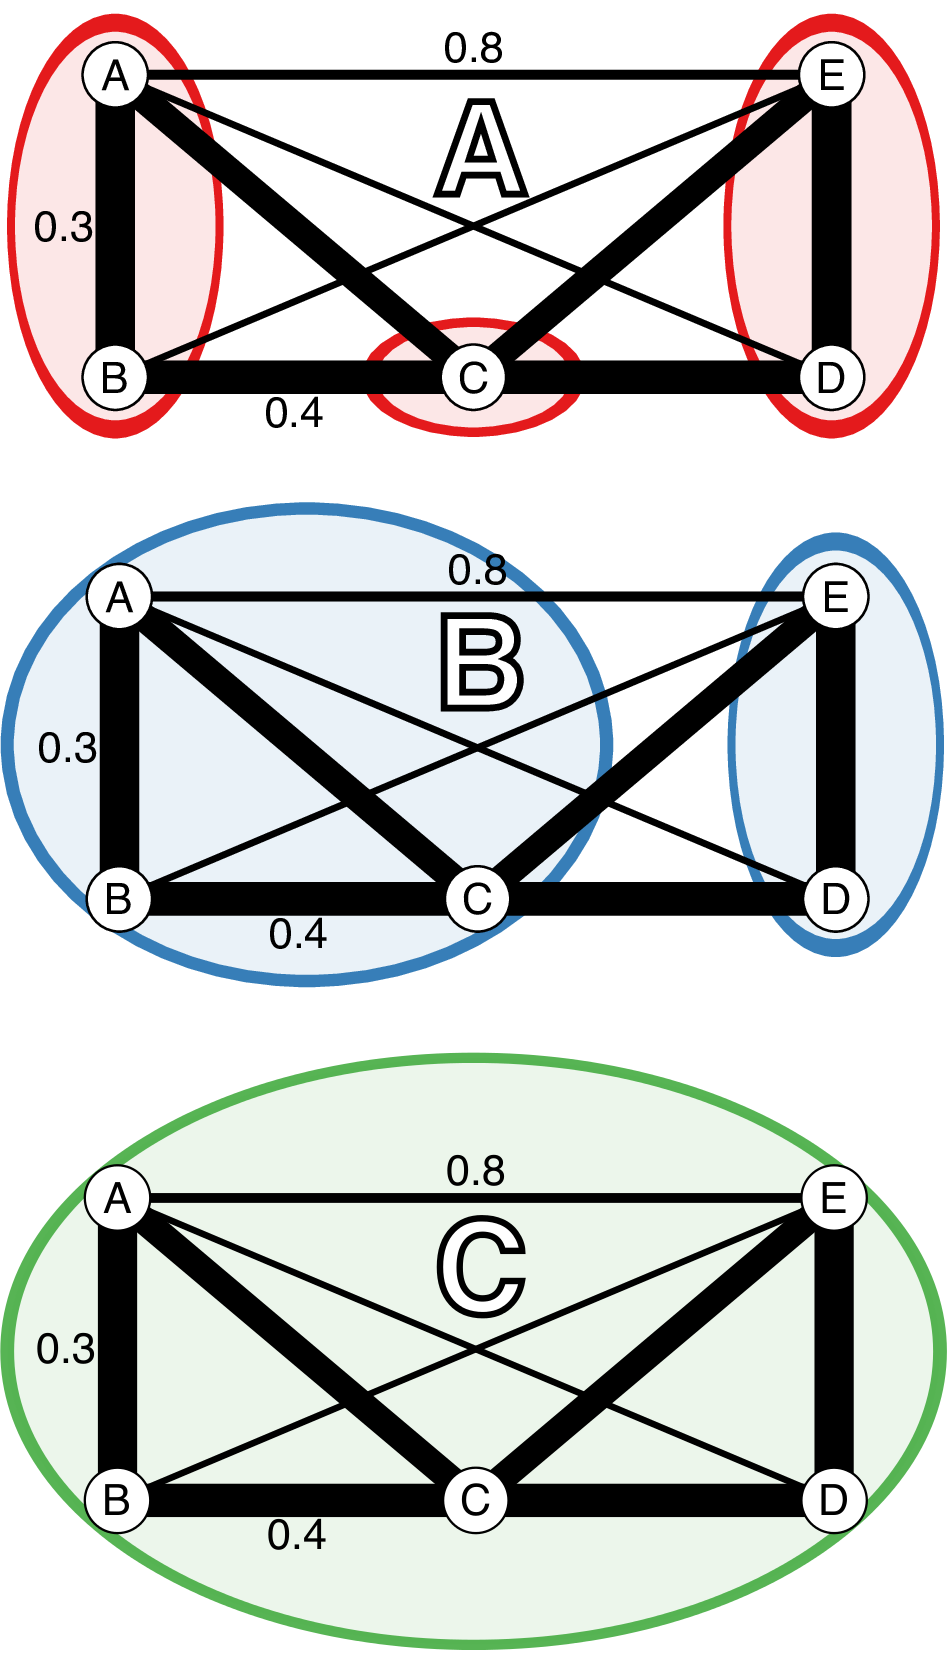
\includegraphics[width=0.5\linewidth]{figure/frontiers/Figure-1} 
  
  }
  
  \caption[Diagrammatic representation of the three clustering algorithms
  implemented in \texttt{mlg.filter}.]{Diagrammatic representation of the three clustering algorithms
  implemented in \texttt{mlg.filter}. (\textbf{A-C}) Represent different
  clustering algorithms on the same imaginary network with a threshold of
  0.451. Edge weights are represented in arbitrary units noted by the line
  thickness and numerical values next to the lines. All outer angles are
  90 degrees, so the un-labeled edge weights can be obtained with simply
  geometry. Colored circles represent clusters of genotypes. (\textbf{A})
  Farthest neighbor clustering does not cluster nodes B and C because
  nodes A and C are more than a distance of 0.451 apart. (\textbf{B})
  UPGMA (average neighbor) clustering clusters nodes A, B, and C together
  because the average distance between them and C is \textless{} 0.451.
  (\textbf{C}) Nearest neighbor clustering clusters all nodes together
  because the minimum distance between them is always \textless{} 0.451.}\label{fig:Figure1}
  \end{figure}
  
  We utilize data from the microbe \emph{Phytophthora infestans} to show
  how the \texttt{mlg.filter} function collapses multilocus genotypes with
  Bruvo's distance assuming a genome addition model (Bruvo \emph{et al.}
  2004). \emph{P. infestans} is the causal agent of potato late blight
  originating from Mexico that spread to Europe in the mid 19th century
  (Yoshida \emph{et al.} 2013; Goss \emph{et al.} 2014). \emph{P.
  infestans} reproduces both clonally and sexually. The clonal lineages of
  \emph{P. infestans} have been formally defined into 18 separate clonal
  lineages using a combination of various molecular methods including AFLP
  and microsatellite markers (Lees \emph{et al.} 2006; Li \emph{et al.}
  2013). For these data, we used \texttt{mlg.filter} to detect all of the
  distance thresholds at which 18 multilocus lineages would be resolved.
  We used these thresholds to define multilocus lineages and create
  contingency tables and dendrograms to determine how well the multilocus
  lineages were detected.
  
  For the \emph{P. infestans} population, the three algorithms were able
  to detect 18 multilocus lineages at different distance thresholds (Fig.
  \ref{fig:Figure-2}). Contingency tables between the described multilocus
  genotypes and the genotypes defined by distance show that most of the 18
  lineages were resolved, except for US-8, which is polytomic (Table
  \ref{pinftable}).
  
  \begin{figure}
  
  {\centering 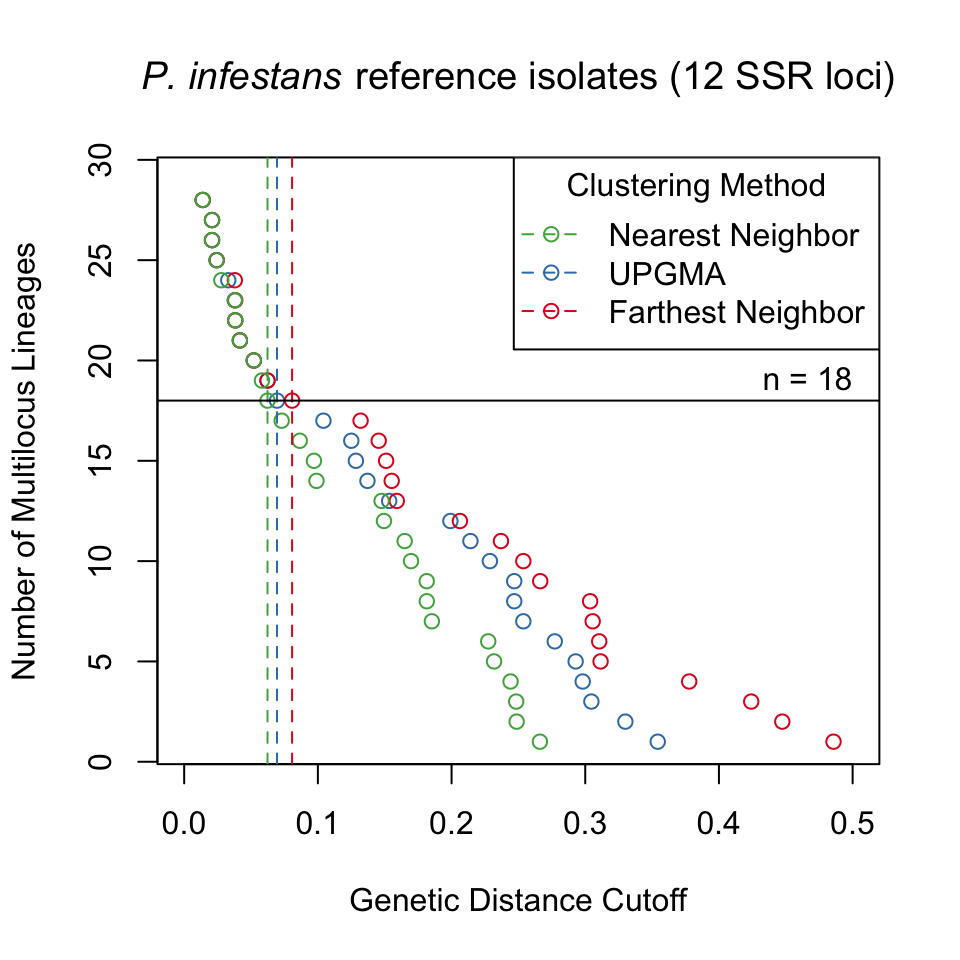
\includegraphics[width=0.8\linewidth]{thesis_files/figure-latex/Figure-2-1} 
  
  }
  
  \caption[Graphical representation of three different clustering algorithms
  collapsing multilocus genotypes for 12 SSR loci from \emph{Phytophthora
  infestans} representing 18 clonal lineages.]{Graphical representation of three different clustering algorithms
  collapsing multilocus genotypes for 12 SSR loci from \emph{Phytophthora
  infestans} representing 18 clonal lineages. The horizontal axis is
  Bruvo's genetic distance assuming the genome addition model. The
  vertical axis represents the number of multilocus lineages observed.
  Each point shows the threshold at which one would observe a given number
  of multilocus genotypes. The horizontal black line represents 18
  multilocus genotypes and vertical dashed lines mark the thresholds used
  to collapse the multilocus genotypes into 18 multilocus lineages.}\label{fig:Figure-2}
  \end{figure}
  
  \begin{sidewaystable}[ph!]
  \centering
  \begin{tabular}{l|cccccccccccccccccc}
    & \textbf{3} & \textbf{4} & \textbf{5} & \textbf{6} & \textbf{8} & \textbf{10} & \textbf{12} & \textbf{15} & \textbf{16} & \textbf{17} & \textbf{18} & \textbf{20} & \textbf{21} & \textbf{22} & \textbf{24} & \textbf{25} & \textbf{27} & \textbf{28} \\ 
    \midrule
  \textbf{B} & . & . & . & . & . & . & . & . & . & . & . & . & . & . & . & 1 & . & . \\ 
    \textbf{C} & . & . & . & . & . & . & . & . & . & . & . & . & . & . & 1 & . & . & . \\ 
    \textbf{D.1} & . & . & . & . & . & . & . & . & . & . & . & . & . & 1 & . & . & . & . \\ 
    \textbf{D.2} & . & . & . & . & . & . & . & . & . & . & . & . & . & 1 & . & . & . & . \\ 
    \textbf{EU-13} & . & . & . & . & . & . & . & . & 1 & . & . & . & . & . & . & . & . & . \\ 
    \textbf{EU-4} & . & . & . & . & . & . & . & . & . & 1 & . & . & . & . & . & . & . & . \\ 
    \textbf{EU-5} & . & . & . & . & . & . & . & . & . & . & 2 & . & . & . & . & . & . & . \\ 
    \textbf{EU-8} & . & . & . & . & . & . & 1 & . & . & . & . & . & . & . & . & . & . & . \\ 
    \textbf{US-11} & . & . & . & . & . & . & . & . & . & . & . & . & . & . & . & . & . & 2 \\ 
    \textbf{US-12} & . & 1 & . & . & . & . & . & . & . & . & . & . & . & . & . & . & . & . \\ 
    \textbf{US-14} & . & . & . & . & . & 1 & . & . & . & . & . & . & . & . & . & . & . & . \\ 
    \textbf{US-17} & . & . & . & . & . & . & . & . & . & . & . & 1 & . & . & . & . & . & . \\ 
    \textbf{US-20} & 2 & . & . & . & . & . & . & . & . & . & . & . & . & . & . & . & . & . \\ 
    \textbf{US-21} & . & . & . & . & . & . & . & . & . & . & . & . & . & . & . & . & 2 & . \\ 
    \textbf{US-22} & . & . & . & . & . & . & . & . & . & . & . & . & 2 & . & . & . & . & . \\ 
    \textbf{US-23} & . & . & . & . & . & . & . & 3 & . & . & . & . & . & . & . & . & . & . \\ 
    \textbf{US-24} & . & . & . & . & 3 & . & . & . & . & . & . & . & . & . & . & . & . & . \\ 
    \textbf{US-8} & . & . & 1 & 1 & . & 2 & . & . & . & . & . & . & . & . & . & . & . & . \\ 
     \bottomrule
  \end{tabular}
  \caption[Contingency table comparing multilocus lineages (MLL)]{Contingency table comparing multilocus lineages (MLL) defined in Li
  \emph{et al.} (2013) and Lees \emph{et al.} (2006) (rows) to MLLs
  inferred from Bruvo's genetic distance (columns) at a threshold of 0.07
  with the average neighbor algorithm (Sokal 1958; Bruvo \emph{et al.}
  2004). Values in the table represent the number of times any given
  inferred MLL matches with a previously defined MLL. For example, in our
  original data set, there were three genotypes previously defined as the
  US-24 MLL. All three genotypes were also determined to cluster into a
  single MLL by filtering. In contrast, US-8 was determined to cluster
  into three different MLLs by filtering.} 
  \label{pinftable}
  \end{sidewaystable}
  
  \newpage
  
  We utilized simulated data to evaluate the effect of sequencing error
  and missing data on MLG calling. We constructed the data using the
  \texttt{glSim} function in \emph{adegenet} (Jombart \& Ahmed 2011) to
  obtain a SNP data set for demonstration. Two diploid data sets were
  created, each with 10k SNPs (25\% structured into two groups) and 200
  samples with 10 ancestral populations of even sizes. Clones were created
  in one data set by marking each sample with a unique identifier and then
  randomly sampling with replacement. It is well documented that reduced-
  representation sequencing can introduce several erroneous calls and
  missing data (Mastretta-Yanes \emph{et al.} 2015). To reflect this, we
  mutated SNPs at a rate of 10\% and inserted an average of 10\% missing
  data for each sample after clones were created, ensuring that no two
  sequences were alike. The number of mutations and missing data per
  sample were determined by sampling from a Poisson distribution with
  \(\lambda = 1000\). After pooling, 20\% of the data set was randomly
  sampled for analysis. Genetic distance was obtained with the function
  \texttt{bitwise.dist}, which calculates the fraction of different sites
  between samples equivalent to Provesti's distance, counting missing data
  as equivalent in comparison (Prevosti \emph{et al.} 1975).
  
  All three filtering algorithms were run with a threshold of 1, returning
  a numeric vector of length \(n - 1\) where each element represented a
  threshold at which two samples/clusters would join. Since each data set
  would have varying distances between samples, the clonal boundary
  threshold was defined as the midpoint of the largest gap between two
  thresholds that collapsed less than 50\% of the data.
  
  Out of the 100 simulations run, we found that across all methods,
  detection of duplicated samples had \(\sim\) 98\% true positive fraction
  and \(\sim\) 0.8\% false positive fraction indicating that this method
  is robust to simulated populations (supplementary materials\footnote{Supplementary
    data available at
    \url{https://github.com/grunwaldlab/supplementary-poppr-2.0}; DOI:
    \href{http://dx.doi.org/10.5281/zenodo.17424}{10.5281/zenodo.17424}}).
  
  \subsection{Minimum Spanning Networks with
  Reticulation}\label{minimum-spanning-networks-with-reticulation}
  
  In its original iteration, \emph{poppr} introduced minimum spanning
  networks that were based on the \emph{igraph} function
  \texttt{minimum.spanning.tree} (Csardi \& Nepusz 2006). This algorithm
  produces a minimum spanning tree with no reticulations where nodes
  represent individual MLGs. In other minimum spanning network programs,
  reticulation is obtained by calculating the minimum spanning tree
  several times and returning the set of all edges included in the trees.
  Due to the way \emph{igraph} has implemented Prim's algorithm, it is not
  possible to utilize this strategy, thus we implemented an internal C
  function to walk the space of minimum spanning trees based on genetic
  distance to connect groups of nodes with edges of equal weight.
  
  To demonstrate the utility of minimum spanning networks with
  reticulation, we used two clonal data sets: the H3N2 flu virus data from
  the \emph{adegenet} package using years of each epidemic as the
  population factor, and \emph{Phytophthora ramorum} data from Nurseries
  and Oregon forests (Jombart \emph{et al.} 2010; Kamvar \emph{et al.}
  2014a). Minimum spanning networks were created with and without
  reticulation using the \emph{poppr} functions \texttt{diss.dist} and
  \texttt{bruvo.msn} for the H3N2 and \emph{P. ramorum} data, respectively
  (Bruvo \emph{et al.} 2004; Kamvar \emph{et al.} 2014b). To detect mlg
  clusters, the infoMAP community detection algorithm was applied with
  10,000 trials as implemented in the R package \emph{igraph} version
  0.7.1 utilizing genetic distance as edge weights and number of samples
  in each MLG as vertex weights (Csardi \& Nepusz 2006; Rosvall \&
  Bergstrom 2008).
  
  To evaluate the results, we compared the number, size, and entropy
  (\(H\)) of the resulting communities as we expect a highly clonal
  organism with low genetic diversity to result in a few, large
  communities. We also created contingency tables of the community
  assignments with the defined populations and used those to calculate
  entropy using Shannon's index with the function \texttt{diversity} from
  the R package \emph{vegan} version 2.2-1 (Shannon 2001; Oksanen \emph{et
  al.} 2015). A low entropy indicates presence of a few large communities
  whereas high entropy indicates presence of many small communities.
  
  The infoMAP algorithm revealed 63 communities with a maximum community
  size of 77 and \(H = 3.56\) for the reticulate network of the H3N2 data
  and 117 communities with a maximum community size of 26 and \(H = 4.65\)
  for the minimum spanning tree. The entropy across years was greatly
  decreased for all populations with the reticulate network compared to
  the minimum spanning tree (Fig. \ref{fig:Figure-3}). Note that the
  reticulated network (Fig. \ref{fig:Figure-3}B) showed patterns
  corresponding with those resulting from a discriminant analysis of
  principal components (Fig. \ref{fig:Figure-3}D) (Jombart \emph{et al.}
  2010).
  
  \begin{figure}
  
  {\centering \includegraphics[width=0.8\linewidth]{figure/frontiers/Figure-3} 
  
  }
  
  \caption[Minimum Spanning Networks with Reticulation]{(\textbf{A-B}) Minimum spanning networks of the hemagglutinin (HA)
  segment of H3N2 viral DNA from the \emph{adegenet} package representing
  flu epidemics from 2001 to 2006 without reticulation (\textbf{A}) and
  with reticulation (\textbf{B}) (Jombart 2008; Jombart \emph{et al.}
  2010). Each node represents a unique multilocus genotype, colors
  represent epidemic year, and edge color represents absolute genetic
  distance. (\textbf{C}) Shannon entropy values for population assignments
  compared with communities determined by the infoMAP algorithm on
  (\textbf{A}) and (\textbf{B}). (\textbf{D}) Graphic reproduced from
  Jombart \emph{et al.} (2010) showing that the 2006 epidemic does not
  cluster neatly with the other years via Discriminant Analysis of
  Principal Components. Horizontal axis represents the first discriminant
  component. Vertical axis represents the second discriminant component.}\label{fig:Figure-3}
  \end{figure}
  
  Graph walking of the reticulated minimum spanning network of \emph{P.
  ramorum} by the infoMAP algorithm revealed 16 communities with a maximum
  community size of 13 and \(H = 2.60\). The un-reticulated minimum
  spanning tree revealed 20 communities with a maximum community size of 7
  and \(H = 2.96\). In the ability to predict Hunter Creek as belonging to
  a single community, the reticulated network was successful whereas the
  minimum spanning tree separated one genotype from that community. The
  entropy for the reticulated network was lower for all populations except
  for the coast population (supplementary materials\footnote{Supplementary
    data available at
    \url{https://github.com/grunwaldlab/supplementary-poppr-2.0}; DOI:
    \href{http://dx.doi.org/10.5281/zenodo.17424}{10.5281/zenodo.17424}}).
  
  \subsection{Bootstrapping}\label{bootstrapping}
  
  Assessing population differentiation through methods such as \(G_{st}\),
  AMOVA, and Mantel tests relies on comparing samples within and across
  populations (Mantel 1967; Nei 1973; Excoffier \emph{et al.} 1992).
  Confidence in distance metrics is related to the confidence in the
  markers to accurately represent the diversity of the data. Especially
  true with microsatellite markers, a single hyper-diverse locus can make
  a population appear to have more diversity based on genetic distance.
  Using a bootstrapping procedure of randomly sampling loci with
  replacement when calculating a distance matrix provides support for
  clades in hierarchical clustering.
  
  Data in genind and genpop objects are represented as matrices with
  individuals in rows and alleles in columns (Jombart 2008). This gives
  the advantage of being able to use R's matrix algebra capabilities to
  efficiently calculate genetic distance. Unfortunately, this also means
  that bootstrapping is a non- trivial task as all alleles at a single
  locus need to be sampled together. To remedy this, we have created an
  internal S4 class called ``bootgen'', which extends the internal ``gen''
  class from \emph{adegenet}. This class can be created from any genind,
  genclone, or genpop object, and allows loci to be sampled with
  replacement. To further facilitate bootstrapping, a function called
  \texttt{aboot}, which stands for ``any boot'', is introduced that will
  bootstrap any genclone, genind, or genpop object with any genetic
  distance that can be calculated from it.
  
  To demonstrate calculating a dendrogram with bootstrap support, we used
  the \emph{poppr} function \texttt{aboot} on population allelic
  frequencies derived from the data set \texttt{microbov} in the
  \emph{adegenet} package with 1000 bootstrap replicates (Laloë \emph{et
  al.} 2007; Jombart 2008). The resulting dendrogram shows bootstrap
  support values \(>50\%\) (Fig. \ref{fig:microboot}) and used the
  following code:
  
  \begin{Shaded}
  \begin{Highlighting}[]
  \KeywordTok{library}\NormalTok{(}\StringTok{"poppr"}\NormalTok{);}
  \KeywordTok{data}\NormalTok{(}\StringTok{"microbov"}\NormalTok{, }\DataTypeTok{package =} \StringTok{"adegenet"}\NormalTok{);}
  \KeywordTok{strata}\NormalTok{(microbov) <-}\StringTok{ }\KeywordTok{data.frame}\NormalTok{(}\KeywordTok{other}\NormalTok{(microbov));}
  \KeywordTok{setPop}\NormalTok{(microbov) <-}\StringTok{ }\ErrorTok{~}\NormalTok{coun/spe/breed;}
  \NormalTok{bov_pop <-}\StringTok{ }\KeywordTok{genind2genpop}\NormalTok{(microbov);}
  
  \KeywordTok{set.seed}\NormalTok{(}\DecValTok{20150428}\NormalTok{);}
  \NormalTok{pop_tree <-}\StringTok{ }\KeywordTok{aboot}\NormalTok{(bov_pop, }\DataTypeTok{sample =} \DecValTok{1000}\NormalTok{, }\DataTypeTok{cutoff =} \DecValTok{50}\NormalTok{);}
  \end{Highlighting}
  \end{Shaded}
  
  \begin{figure}
  
  {\centering 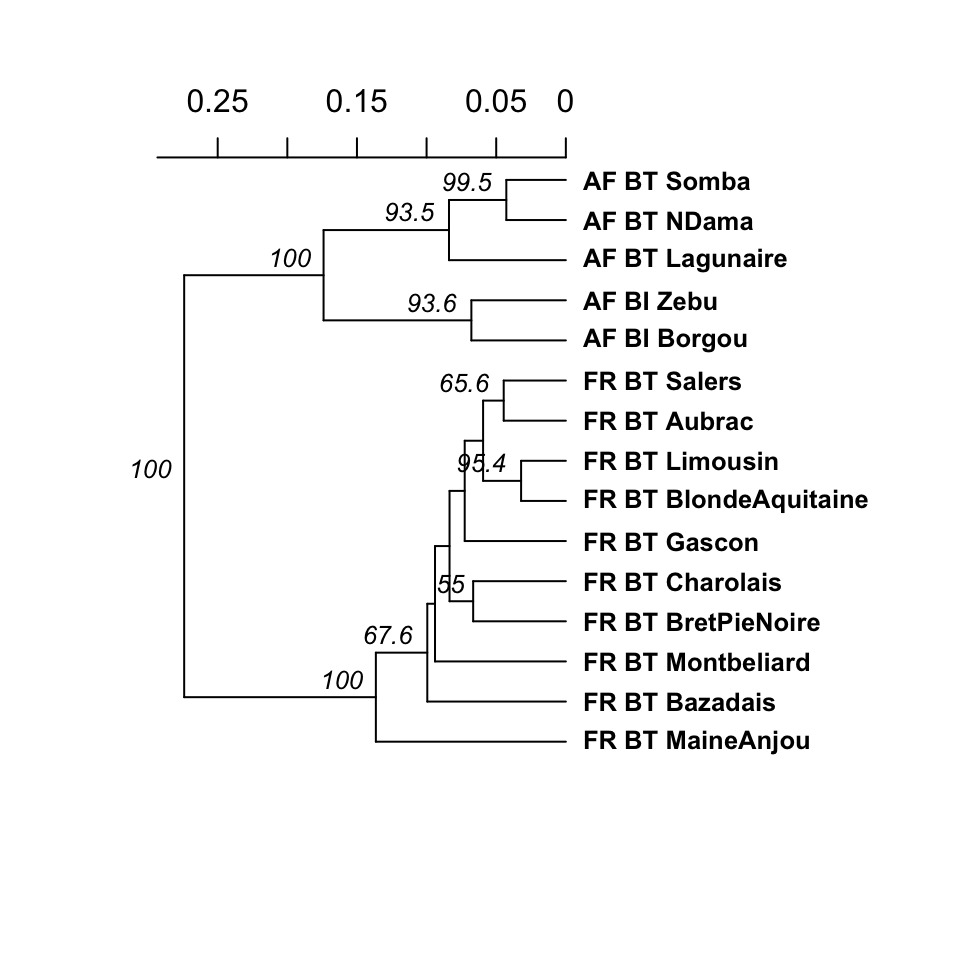
\includegraphics[width=0.8\linewidth]{thesis_files/figure-latex/microboot-1} 
  
  }
  
  \caption[UPGMA dendrogram generated from Nei's genetic distance]{UPGMA dendrogram generated from Nei's genetic distance on 15 breeds of
  \emph{Bos taurus} (BT) or \emph{Bos indicus} (BI) from Africa (AF) or
  France (FR). These data are from Laloë \emph{et al.} (2007). Node labels
  represent bootstrap support \(>50\%\) out of 1,000 bootstrap replicates.}\label{fig:microboot}
  \end{figure}
  
  \subsection{Genotype Accumulation
  Curve}\label{genotype-accumulation-curve}
  
  Analysis of population genetics of clonal organisms often borrows from
  ecological methods such as analysis of diversity within populations
  (Milgroom 1996; Grünwald \emph{et al.} 2003; Arnaud-Hanod \emph{et al.}
  2007). When choosing markers for analysis, it is important to make sure
  that the observed diversity in your sample will not appreciably increase
  if an additional marker is added (Arnaud-Hanod \emph{et al.} 2007). This
  concept is analogous to a species accumulation curve, obtained by
  rarefaction. The genotype accumulation curve in \emph{poppr} is
  implemented in the function \texttt{genotype\_curve}. The curve is
  constructed by randomly sampling \(x\) loci and counting the number of
  observed MLGs. This repeated \(r\) times for 1 locus up to \(n-1\) loci,
  creating \(n-1\) distributions of observed MLGs.
  
  The following code example demonstrates the genotype accumulation curve
  for data from Everhart \& Scherm (2015) showing that these data reach a
  small plateau and have a greatly decreased variance with 12 markers,
  indicating that there are enough markers such that adding more markers
  to the analysis will not create very many new genotypes (Fig.
  \ref{fig:moniliniacurve}).
  
  \begin{Shaded}
  \begin{Highlighting}[]
  \KeywordTok{library}\NormalTok{(}\StringTok{"poppr"}\NormalTok{);}
  \KeywordTok{library}\NormalTok{(}\StringTok{"ggplot2"}\NormalTok{);}
  \KeywordTok{data}\NormalTok{(}\StringTok{"monpop"}\NormalTok{, }\DataTypeTok{package =} \StringTok{"poppr"}\NormalTok{);}
  
  \KeywordTok{set.seed}\NormalTok{(}\DecValTok{20150428}\NormalTok{);}
  \KeywordTok{genotype_curve}\NormalTok{(monpop, }\DataTypeTok{sample =} \DecValTok{1000}\NormalTok{);}
  \NormalTok{p <-}\StringTok{ }\KeywordTok{last_plot}\NormalTok{() +}\StringTok{ }\KeywordTok{theme_bw}\NormalTok{();   }\CommentTok{# get the last plot}
  \NormalTok{p +}\StringTok{ }\KeywordTok{geom_smooth}\NormalTok{(}\KeywordTok{aes}\NormalTok{(}\DataTypeTok{group =} \DecValTok{1}\NormalTok{)); }\CommentTok{# plot with a trendline}
  \end{Highlighting}
  \end{Shaded}
  
  \begin{figure}
  
  {\centering 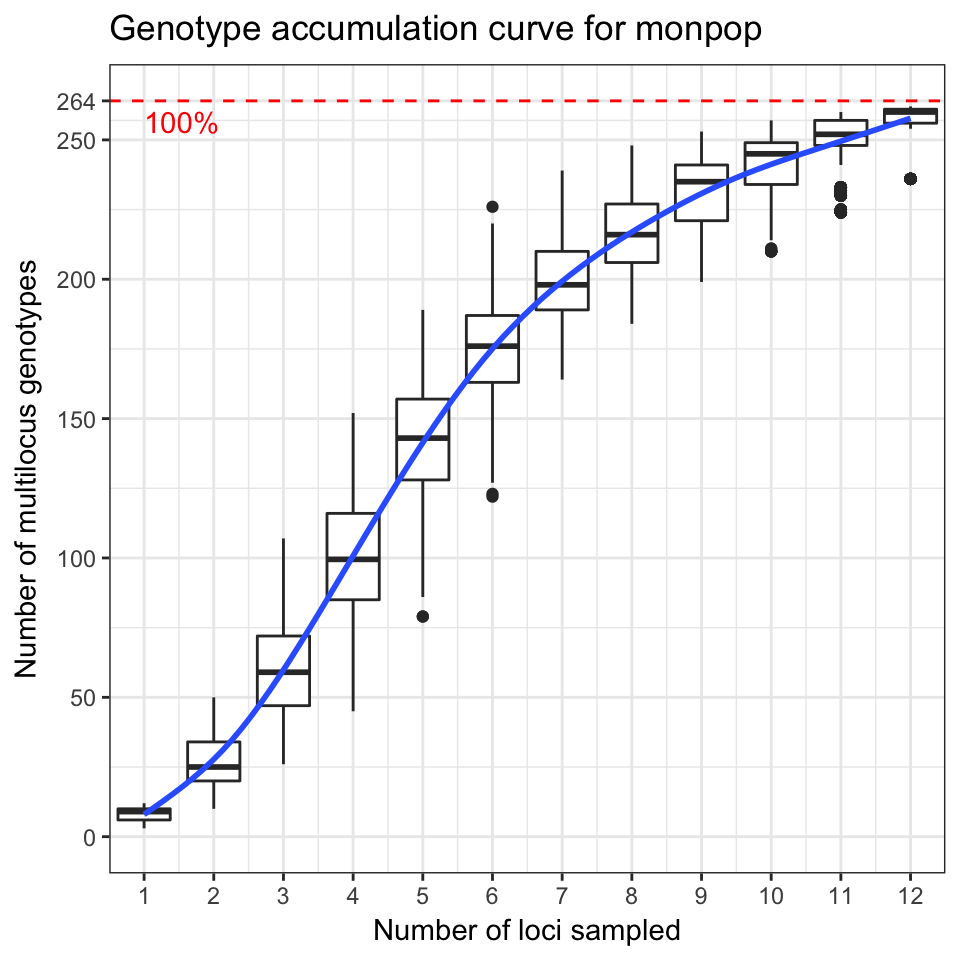
\includegraphics[width=0.8\linewidth]{thesis_files/figure-latex/moniliniacurve-1} 
  
  }
  
  \caption[Genotype accumulation curve]{Genotype accumulation curve for 694 isolates of the peach brown rot
  pathogen, \emph{Monilinia fructicola} genotyped over 13 loci from
  Everhart \& Scherm (2015). The horizontal axis represents the number of
  loci randomly sampled without replacement up to \emph{n - 1} loci, the
  vertical axis shows the number of multilocus genotypes observed, up to
  262, the number of unique multilocus genotypes in the data set. The red
  dashed line represents 90\% of the total observed multilocus genotypes.
  A trendline (blue) has been added using the \emph{ggplot2} function
  \texttt{stat\_smooth}.}\label{fig:moniliniacurve}
  \end{figure}
  
  \subsection{Index of association}\label{index-of-association-1}
  
  The index of association (\(I_A\)) is a measure of multilocus linkage
  disequilibrium that is most often used to detect clonal reproduction
  within organisms that have the ability to reproduce via sexual or
  asexual processes (Brown \emph{et al.} 1980; Smith \emph{et al.} 1993;
  Milgroom 1996). It was standardized in 2001 as \(\bar{r}_d\) by Agapow
  \& Burt (2001) to address the issue of scaling with increasing number of
  loci. This metric is typically applied to traditional dominant and
  co-dominant markers such as AFLPs, SNPs, or microsatellite markers. With
  the advent of high throughput sequencing, SNP data is now available in a
  genome-wide context and in very large matrices including thousands of
  SNPs. For this reason, we devised two approaches using the index of
  association for large numbers of markers typical for population genomic
  studies. Both functions utilize \emph{adegenet}'s ``genlight'' object
  class, which efficiently stores 8 binary alleles in a single byte
  (Jombart \& Ahmed 2011). As calculation of the \(\bar{r}_d\) requires
  distance matrices of absolute number of differences, we utilize a
  function that calculates these distances directly from the compressed
  data called \texttt{bitwise.dist}.
  
  The first approach is a sliding window analysis implemented in the
  function \texttt{win.ia}. It utilizes the position of markers in the
  genome to calculate \(\bar{r}_d\) among any number of SNPs found within
  a user-specified windowed region. It is important that this calculation
  utilize \(\bar{r}_d\) as the number of loci will be different within
  each window (Agapow \& Burt 2001). This approach would be suited for a
  quick calculation of linkage disequilibrium across the genome that can
  detect potential hotspots of LD that could be investigated further with
  more computationally intensive methods assuming that the number of
  samples \textless{}\textless{} the number of loci.
  
  As it would necessarily focus on loci within a short section of the
  genome that may or may not be recombining, a sliding window approach
  would not be good for utilizing \(\bar{r}_d\) as a test for clonal
  reproduction. A remedy for this is implemented in the function
  \texttt{samp.ia}, which will randomly sample \(m\) loci, calculate
  \(\bar{r}_d\), and repeat \(r\) times, thus creating a distribution of
  expected values of \(\bar{r}_d\).
  
  To demonstrate the sliding window and random sampling of \(\bar{r}_d\)
  with respect to clonal populations, we simulated two populations
  containing 1,100 neutral SNPs for 100 diploid individuals under the same
  initial seed. One population had individuals randomly sampled with
  replacement, representing the clonal population. After sampling, both
  populations had 5\% random error and 1\% missing data independently
  propagated across all samples. On average, we obtained a higher value of
  \(\bar{r}_d\) for the clonal population compared to the sexual
  population for both methods (Fig. \ref{fig:Figure-6}).
  
  \begin{figure}
  
  {\centering 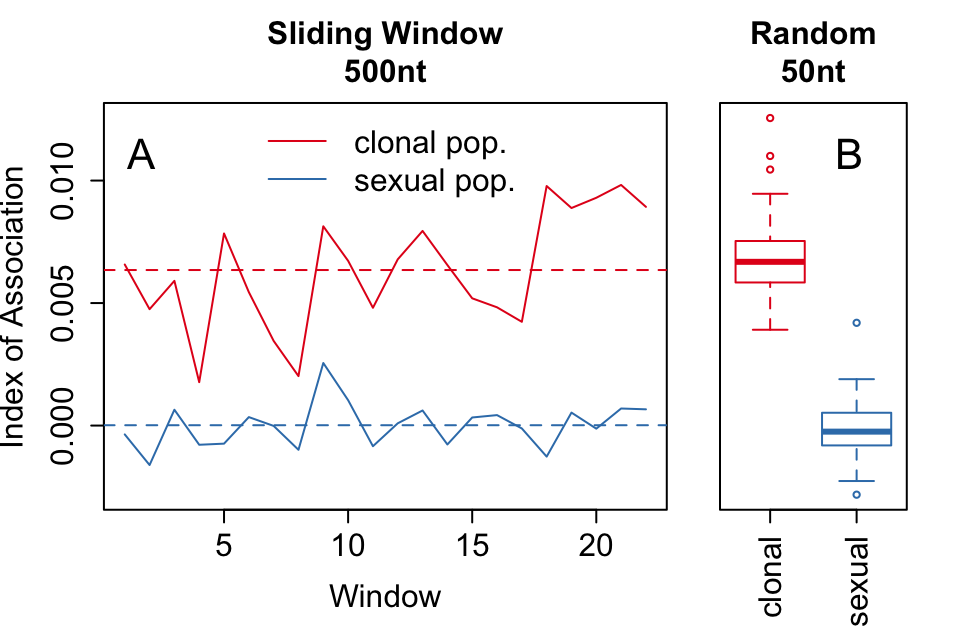
\includegraphics[width=0.8\linewidth]{thesis_files/figure-latex/Figure-6-1} 
  
  }
  
  \caption[Sliding window analysis of the standardized index of association
  (\(\bar{r}_d\))]{\textbf{(A)} Sliding window analysis of the standardized index of
  association (\(\bar{r}_d\)) across a simulated \(1.1 \times 10^4\) nt
  chromosome containing 1,100 variants among 100 individuals. Each window
  analyzed variants within 500nt chunks. The black line refers to the
  clonal and the blue line to the sexual populations. \textbf{(B)}
  boxplots showing 100 random samples of 50 variants to calculate a
  distribution of \(\bar{r}_d\) for the clonal (red) and sexual (blue)
  populations. Each box is centered around the mean, with whiskers
  extending out to 1.5 times the interquartile range. The median is
  indicated by the center line. \textbf{(A)} and \textbf{(B)} are plotted
  on the same y-axis.}\label{fig:Figure-6}
  \end{figure}
  
  \subsection{Data format updates: population strata and
  hierarchies}\label{data-format-updates-population-strata-and-hierarchies}
  
  Assessments of population structure through methods such as hierarchical
  \(F_{st}\) (Goudet 2005) and AMOVA (Michalakis \& Excoffier 1996)
  require hierarchical sampling of populations across space or time (Linde
  \emph{et al.} 2002; Grünwald \& Hoheisel 2006; Everhart \& Scherm 2015).
  With clonal organisms, basic practice has been to clone-censor data to
  avoid downward bias in diversity due to duplicated genotypes that may or
  may not represent different samples (Milgroom 1996). This correction
  should be performed with respect to a population hierarchy to accurately
  reflect the biology of the organism. Traditional data structures for
  population genetic data in most analysis tools allow for only one level
  of hierarchical definition. The investigator thus had to provide the
  data set for analysis at each hierarchical level.
  
  To facilitate handling hierarchical and mutlilocus genotypic metadata,
  \emph{poppr} version 1.1 introduced a new S4 data object called
  ``genclone'', extending \emph{adegenet}'s ``genind'' object (Kamvar and
  Grünwald, unpublished). The genclone object formalized the definitions
  of multilocus genotypes and population hierarchies by adding two slots
  called ``mlg'' and ``hierarchy'' that carried a numeric vector and a
  data frame, respectively. These new slots allow for increased efficiency
  and ease of use by allowing these metadata to travel with the genetic
  data. The hierarchy slot in particular contains a data frame where each
  column represents a separate hierarchical level. This is then used to
  set the population factor of the data by supplying a hierarchical
  formula containing one or more column names of the data frame in the
  hierarchy slot.
  
  The functionality represented by the hierarchy slot has now been
  migrated from the \emph{poppr} to the \emph{adegenet} package version
  2.0 to allow hierarchical analysis in \emph{adegenet}, \emph{poppr}, and
  other dependent packages. The prior \emph{poppr} \texttt{hierarchy} slot
  and methods have now been renamed \texttt{strata} in \emph{adegenet}. A
  short example of the utility of these methods can be seen in the code
  segment under \textbf{Bootstrapping}, above. This migration provides end
  users with a broader ability to analyze data hierarchically in R across
  packages.
  
  \section{Availability}\label{availability}
  
  As of this writing, the \emph{poppr} R package version 2.0 containing
  all of the features described here is located at
  \url{https://github.com/grunwaldlab/poppr/tree/2.0-rc}. It is necessary
  to install \emph{adegenet} 2.0 before installing \emph{poppr}. It can be
  found at \url{https://github.com/thibautjombart/adegenet}. Both of these
  can be installed via the R package \emph{devtools} (Wickham \& Chang
  2015). More information and example code can be found in the
  supplementary materials\footnote{Supplementary data available at
    \url{https://github.com/grunwaldlab/supplementary-poppr-2.0}; DOI:
    \href{http://dx.doi.org/10.5281/zenodo.17424}{10.5281/zenodo.17424}}.
  
  \subsection{Requirements}\label{requirements}
  
  \begin{itemize}
  \tightlist
  \item
    R version 3.0 or better
  \item
    A C compiler. For windows, it can be obtained via Rtools
    (\url{http://cran.r-project.org/bin/windows/Rtools/}). On OSX, it can
    be obtained via Xcode. For parallel support, gcc version 4.6 or better
    is needed.
  \end{itemize}
  
  \newpage
  
  \subsection{Installation}\label{installation}
  
  From within R, \emph{poppr} can be installed via:
  
  \begin{Shaded}
  \begin{Highlighting}[]
  \KeywordTok{install.packages}\NormalTok{(}\StringTok{"devtools"}\NormalTok{)}
  \KeywordTok{library}\NormalTok{(}\StringTok{"devtools"}\NormalTok{)}
  \KeywordTok{install_github}\NormalTok{(}\StringTok{"thibautjombart/adegenet"}\NormalTok{)}
  \KeywordTok{install_github}\NormalTok{(}\StringTok{"grunwaldlab/poppr@2.0-rc"}\NormalTok{)}
  \end{Highlighting}
  \end{Shaded}
  
  Several population genetics packages in R are currently going through a
  major upgrade following the 2015 R hackathon on population genetics
  (\url{https://github.com/NESCent/r-popgen-hackathon}) and have not yet
  been updated in CRAN. We will upload \emph{poppr} 2.0 to CRAN once all
  other reverse dependent packages have been updated.
  
  \section{Discussion}\label{discussion-1}
  
  Given low cost and high throughput of current sequencing technologies we
  are entering a new era of population genetics where large SNP data sets
  with thousands of markers are becoming available for large populations
  in a genome- wide context. This data provides new possibilities and
  challenges for population genetic analyses. We provide novel tools that
  enable analysis of this data in R with a particular emphasis on clonal
  organisms.
  
  Particularly useful is the implementation of \(\bar{r}_d\) in a genomic
  context (Agapow \& Burt 2001). Random sampling of loci across the genome
  can give an expected distribution of \(\bar{r}_d\), which is expected to
  have a mean of zero for panmictic populations. This metric is not
  affected by the number of loci sampled, is model free, and has the
  ability to detect population structure. \(\bar{r}_d\) is also
  implemented for sliding window analyses that are useful to detect
  candidate regions of linkage disequilibrium for further analysis.
  
  Clustering multilocus genotypes into multilocus lineages based on
  genetic distances is a non-trivial task given large SNP data sets.
  Moreover, this has not previously been implemented for genomic data for
  clonal populations. Clonal assignment has previously been available in
  the programs \textsc{GenClone} and \textsc{Genodive} for classical
  markers (Meirmans \& Van Tienderen 2004; Arnaud-Hanod \emph{et al.}
  2007). Our method with \texttt{mlg.filter} builds upon this idea and
  allows the user to choose between three different approaches for
  clustering MLGs. The choice of clustering algorithm has an impact on the
  data (Fig. \ref{fig:Figure1}, \ref{fig:Figure-2}), where for example a
  genetic distance cutoff of 0.1 would be the difference between 14
  multilocus lineages (MLLs) and 17 MLLs for nearest neighbor and UPGMA
  clustering, respectively (Fig. \ref{fig:Figure-2}). The option to choose
  the clustering algorithm gives the user the ability to choose what is
  biologically relevant to their populations. While there is not one
  optimal procedure for defining boundaries in clonal lineages, our tool
  provides a means of exploring the potential MLG or MLL boundary space.
  
  Minimum spanning networks are a useful tool to analyze the relationships
  between individuals in a population, because it reduces the complexity
  of a distance matrix to the connections that are strongest. By default,
  these networks are drawn without reticulations, but for clonal organisms
  where many of the connections between samples are equivalent, the
  minimum spanning network appears as a chain and reduces the information
  that can be communicated. This is problematic because the ability to
  detect population structure with one instance of a minimum spanning
  network is limited. Adding reticulation into the minimum spanning
  network thus presents all equivalent connections and allows population
  structure to be more readily detectable. As shown in Fig.
  \ref{fig:Figure-3}, population structure is apparent both visually and
  by graph community detection algorithms such as the infoMAP algorithm
  (Rosvall \& Bergstrom 2008). Additionally, the current implementation in
  \emph{poppr} has been successfully used in analyses such as
  reconstruction of the \emph{P. ramorum} epidemic in Oregon forests
  (Kamvar \emph{et al.} 2014a, 2015).
  
  \emph{Poppr} 2.0 is open source and available on GitHub. Members of the
  community are invited to contribute by raising issues or pull requests
  on our repository at \url{https://github.com/grunwaldlab/poppr/issues}.
  
  \newpage
  
  \section{Acknowledgements}\label{acknowledgements-1}
  
  We thank Ignazio Carbone for discussions on the index of association;
  David Cooke, Sanmohan Baby, and Jens Hansen for beta testing; and
  Thibaut Jombart for allowing us to incorporate the \texttt{strata} slot
  and related methods in \emph{adegenet}. We also thank all the members of
  the 2015 R hackathon on population genetics in Durham, NC for their
  advice and input (\url{https://github.com/NESCent/r-popgen-hackathon}).
  This work was supported in part by US Department of Agriculture (USDA)
  Agricultural Research Service Grant 5358-22000-039-00D, USDA National
  Institute of Food and Agriculture Grant 2011-68004-30154, USDA APHIS,
  the USDA-ARS Floriculture Nursery Initiative, and the USDA-Forest
  Service Forest Health Monitoring Program (to NJG).
  
  \chapter{\texorpdfstring{{[}Tentative Title{]} Population Dynamics of
  the Plant Pathogen \emph{Phytophthora syringae} in Oregon
  Nurseries}{{[}Tentative Title{]} Population Dynamics of the Plant Pathogen Phytophthora syringae in Oregon Nurseries}}\label{tentative-title-population-dynamics-of-the-plant-pathogen-phytophthora-syringae-in-oregon-nurseries}
  
  \section{Abstract}\label{abstract-3}
  
  \section{Introduction}\label{introduction-3}
  
  \emph{Phytophthora syringae} is the most important species affecting
  ornamentals produced in the Pacific Northwest. Recent nursery sampling
  efforts, aimed at characterizing the diversity of \emph{Phytophthoras}
  within Oregon nurseries, have revealed the species \emph{P. syringae} to
  be among the most abundant taxa found in the nurseries surveyed (Parke
  \emph{et al.} 2014). \emph{P. syringae} is adapted to cold weather and
  grows best in the cool, wet fall, winter and spring and is least active
  in summer (Erwin \emph{et al.} 1996). Like \emph{P. ramorum}, it has a
  wide host range including \emph{Rhododendron}, \emph{Camellia},
  \emph{Malus}, and many other taxa. It has the capability for
  outcrossing, self-fertilizing, and reproducing clonally. This pathogen
  has been found globally since 1881 and is problematic on woody
  ornamentals such as crabapple (\emph{Malus spp.}), as it causes
  unsightly cankers that make the plant unsellable (Erwin \emph{et al.}
  1996). While the ecology of this pathogen has been studied to some
  degree, very little is known about the demographic history and
  population structure on a local and global scale.
  
  \chapter{{[}Tentative Title{]} The Effect of Population Dynamics, Sample
  Size, and Marker Choice on the Index of
  Association}\label{tentative-title-the-effect-of-population-dynamics-sample-size-and-marker-choice-on-the-index-of-association}
  
  \section{Abstract}\label{abstract-4}
  
  TBD\ldots{}
  
  \section{Introduction}\label{introduction-4}
  
  \begin{itemize}
  \tightlist
  \item
    Population Genetics of partially clonal organisms
  
    \begin{itemize}
    \tightlist
    \item
      This has been studied in the past (Orive 1993; Smith \emph{et al.}
      1993; Balloux \emph{et al.} 2003; de Meeûs \& Balloux 2004)
    \item
      The index of association (Brown \emph{et al.} 1980; Smith \emph{et
      al.} 1993; Agapow \& Burt 2001)
    \item
      In de Meeûs \& Balloux (2004), it was shown that \(\bar{r}_d\) has a
      high variance in clonal populations and Smith \emph{et al.} (1993)
      showed that it's affected by population structure.
    \end{itemize}
  \item
    Methods for assessing level of clonal reproduction (CloNcaSe) (Ali
    \emph{et al.} 2016)
  
    \begin{itemize}
    \tightlist
    \item
      This only works for populations with discrete generations with an
      observable sexual stage.
    \end{itemize}
  \item
    Limitations of previous studies
  
    \begin{itemize}
    \tightlist
    \item
      No HTS markers
    \item
      Significance tests are routinely performed via permutation analysis,
      but could not be performed due to software limitations (Burt
      \emph{et al.} 1996; de Meeûs \& Balloux 2004)
    \end{itemize}
  \item
    Objectives
  
    \begin{enumerate}
    \def\labelenumi{\arabic{enumi}.}
    \tightlist
    \item
      Analyze mixtures of clonal populations to assess effect of sampling
      multiple clonal populations
    \item
      Re-analyze rates of sexual reproduction to confirm previous study
    \item
      Assess significance tests for \(\bar{r}_d\)
    \end{enumerate}
  \end{itemize}
  
  \section{Methods}\label{methods}
  
  All simulations were performed with the python package simuPOP version
  1.1.7 in python version 3.4. For each scenario, 100 simulations with 10
  replicates were created with a census size of 10,000 individuals evolved
  over 10,000 generations. From each replicate, 10, 25, 50, and 100
  individuals were sampled without replacement for downstream analysis.
  
  \subsection{Microsatellite Simulation}\label{microsatellite-simulation}
  
  Each population was simulated with 20 co-dominant loci containing 6 to
  10 alleles with frequencies drawn from a uniform distribution and
  normalized. Before mating, mutations occurred at each locus at a rate of
  1e-5 mutations/generation.
  
  \subsection{Microsatellite Analysis}\label{microsatellite-analysis}
  
  The standardized index of association (\(\bar{r}_d\)) was calculated in
  R version 3.2 with the package \emph{poppr} version 2.2.1 using the
  function \texttt{ia()} within custom scripts (supplementary
  information). Tests for significance were performed by randomly
  permuting the alleles at each locus independently and then assessing
  \(\bar{r}_d\). This was done 999 times for each replicate population.
  The p-values reflect the proportion of observations greater than the
  observed statistic.
  
  \subsection{GBS Simulations}\label{gbs-simulations}
  
  Simulations of 10,000 binary loci at intervals of 1 Mbp over 100
  chromosomal fragments were simulated with a mutation rate of 1e-5
  mutations per generation and a recombination rate of 1e-5 for sexually
  recombining populations.
  
  \backmatter
  
  \chapter{References}\label{references}
  
  \noindent
  
  \setlength{\parindent}{-0.20in} \setlength{\leftskip}{0.20in}
  \setlength{\parskip}{8pt}
  
  \hypertarget{refs}{}
  \hypertarget{ref-Agapowux5f2001}{}
  Agapow P-M, Burt A (2001) Indices of multilocus linkage disequilibrium.
  \emph{Molecular Ecology Notes}, \textbf{1}, 101--102.
  
  \hypertarget{ref-ali2016cloncase}{}
  Ali S, Soubeyrand S, Gladieux P \emph{et al.} (2016) Cloncase:
  Estimation of sex frequency and effective population size by clonemate
  resampling in partially clonal organisms. \emph{Molecular Ecology
  Resources}.
  
  \hypertarget{ref-anderson1995clonality}{}
  Anderson JB, Kohn LM (1995) Clonality in soilborne, plant-pathogenic
  fungi. \emph{Annual review of phytopathology}, \textbf{33}, 369--391.
  
  \hypertarget{ref-arnaud2007standardizing}{}
  Arnaud-Hanod S, Duarte CM, Alberto F, Serrão EA (2007) Standardizing
  methods to address clonality in population studies. \emph{Molecular
  Ecology}, \textbf{16}, 5115--5139.
  
  \hypertarget{ref-baldauf2003deep}{}
  Baldauf S (2003) The deep roots of eukaryotes. \emph{Science},
  \textbf{300}, 1703--1706.
  
  \hypertarget{ref-balloux2003population}{}
  Balloux F, Lehmann L, de Meeûs T (2003) The population genetics of
  clonal and partially clonal diploids. \emph{Genetics}, \textbf{164},
  1635--1644.
  
  \hypertarget{ref-brown1980multilocus}{}
  Brown A, Feldman M, Nevo E (1980) Multilocus structure of natural
  populations of \emph{Hordeum spontaneum}. \emph{Genetics}, \textbf{96},
  523--536.
  
  \hypertarget{ref-bruvo2004simple}{}
  Bruvo R, Michiels NK, D'Souza TG, Schulenburg H (2004) A simple method
  for the calculation of microsatellite genotype distances irrespective of
  ploidy level. \emph{Molecular Ecology}, \textbf{13}, 2101--2106.
  
  \hypertarget{ref-burt1996molecular}{}
  Burt A, Carter DA, Koenig GL, White TJ, Taylor JW (1996) Molecular
  markers reveal cryptic sex in the human pathogen \emph{Coccidioides
  immitis}. \emph{Proceedings of the National Academy of Sciences},
  \textbf{93}, 770--773.
  
  \hypertarget{ref-butlin2000virgin}{}
  Butlin RK (2000) Virgin rotifers. \emph{Trends in Ecology \& Evolution},
  \textbf{15}, 389--390.
  
  \hypertarget{ref-chakarov2015apparent}{}
  Chakarov N, Linke B, Boerner M \emph{et al.} (2015) Apparent
  vector-mediated parent-to-offspring transmission in an avian
  malaria-like parasite. \emph{Molecular ecology}, \textbf{24},
  1355--1363.
  
  \hypertarget{ref-cooke2012genome}{}
  Cooke DE, Cano LM, Raffaele S \emph{et al.} (2012) Genome analyses of an
  aggressive and invasive lineage of the Irish potato famine pathogen.
  \emph{PLoS pathogens}, \textbf{8}, e1002940.
  
  \hypertarget{ref-csardi2006igraph}{}
  Csardi G, Nepusz T (2006) The igraph software package for complex
  network research. \emph{InterJournal}, \textbf{Complex Systems}, 1695.
  
  \hypertarget{ref-dagum1998openmp}{}
  Dagum L, Menon R (1998) OpenMP: An industry standard API for
  shared-memory programming. \emph{Computational Science \& Engineering,
  IEEE}, \textbf{5}, 46--55.
  
  \hypertarget{ref-davey2010rad}{}
  Davey JW, Blaxter ML (2010) RADSeq: Next-generation population genetics.
  \emph{Briefings in Functional Genomics}, \textbf{9}, 416--423.
  
  \hypertarget{ref-davey2011genome}{}
  Davey JW, Hohenlohe PA, Etter PD \emph{et al.} (2011) Genome-wide
  genetic marker discovery and genotyping using next-generation
  sequencing. \emph{Nature Reviews Genetics}, \textbf{12}, 499--510.
  
  \hypertarget{ref-de2004clonal}{}
  de Meeûs T, Balloux F (2004) Clonal reproduction and linkage
  disequilibrium in diploids: A simulation study. \emph{Infection,
  genetics and evolution}, \textbf{4}, 345--351.
  
  \hypertarget{ref-dobzhansky2013nothing}{}
  Dobzhansky T (1973) Nothing in biology makes sense except in the light
  of evolution. \emph{The American Biology Teacher}, \textbf{75}, 87--91.
  
  \hypertarget{ref-elshire2011robust}{}
  Elshire RJ, Glaubitz JC, Sun Q \emph{et al.} (2011) A robust, simple
  genotyping-by-sequencing (GBS) approach for high diversity species.
  \emph{PloS one}, \textbf{6}, e19379.
  
  \hypertarget{ref-erwin1996phytophthora}{}
  Erwin DC, Ribeiro OK, others (1996) \emph{Phytophthora diseases
  worldwide}. American Phytopathological Society (APS Press), St. Paul,
  Minnesota, USA.
  
  \hypertarget{ref-everhart2014fine}{}
  Everhart S, Scherm H (2015) Fine-scale genetic structure of
  \emph{Monilinia fructicola} during brown rot epidemics within individual
  peach tree canopies. \emph{Phytopathology}, \textbf{105}, 542--549.
  
  \hypertarget{ref-excoffier1992analysis}{}
  Excoffier L, Smouse PE, Quattro JM (1992) Analysis of molecular variance
  inferred from metric distances among DNA haplotypes: Application to
  human mitochondrial DNA restriction data. \emph{Genetics}, \textbf{131},
  479--491.
  
  \hypertarget{ref-Falush01082003}{}
  Falush D, Stephens M, Pritchard JK (2003) Inference of population
  structure using multilocus genotype data: Linked loci and correlated
  allele frequencies. \emph{Genetics}, \textbf{164}, 1567--1587.
  
  \hypertarget{ref-goss2009population}{}
  Goss EM, Larsen M, Chastagner GA, Givens DR, Grünwald NJ (2009)
  Population genetic analysis infers migration pathways of
  \emph{Phytophthora ramorum} in US nurseries. \emph{PLoS Pathogens},
  \textbf{5}, e1000583.
  
  \hypertarget{ref-goss2014irish}{}
  Goss EM, Tabima JF, Cooke DE \emph{et al.} (2014) The Irish potato
  famine pathogen \emph{Phytophthora infestans} originated in central
  Mexico rather than the Andes. \emph{Proceedings of the National Academy
  of Sciences}, \textbf{111}, 8791--8796.
  
  \hypertarget{ref-goudet2005hierfstat}{}
  Goudet J (2005) Hierfstat, a package for R to compute and test
  hierarchical F-statistics. \emph{Molecular Ecology Notes}, \textbf{5},
  184--186.
  
  \hypertarget{ref-gross2014population}{}
  Gross A, Hosoya T, Queloz V (2014) Population structure of the invasive
  forest pathogen \emph{Hymenoscyphus pseudoalbidus}. \emph{Molecular
  ecology}, \textbf{23}, 2943--2960.
  
  \hypertarget{ref-grunwald2011evolution}{}
  Grünwald NJ, Goss EM (2011) Evolution and population genetics of exotic
  and re-emerging pathogens: Novel tools and approaches. \emph{Annual
  Review of Phytopathology}, \textbf{49}, 249--267.
  
  \hypertarget{ref-grunwald2006hierarchical}{}
  Grünwald NJ, Hoheisel G-A (2006) Hierarchical analysis of diversity,
  selfing, and genetic differentiation in populations of the oomycete
  \emph{Aphanomyces euteiches}. \emph{Phytopathology}, \textbf{96},
  1134--1141.
  
  \hypertarget{ref-grunwald2003analysis}{}
  Grünwald NJ, Goodwin SB, Milgroom MG, Fry WE (2003) Analysis of
  genotypic diversity data for populations of microorganisms.
  \emph{Phytopathology}, \textbf{93}, 738--46.
  
  \hypertarget{ref-grunwald2008phytophthora}{}
  Grünwald NJ, Goss EM, Press CM (2008) \emph{Phytophthora ramorum}: a
  pathogen with a remarkably wide host range causing sudden oak death on
  oaks and ramorum blight on woody ornamentals. \emph{Molecular Plant
  Pathology}, \textbf{9}, 729--740.
  
  \hypertarget{ref-grunwald2011phytophthora}{}
  Grünwald NJ, Martin FN, Larsen MM \emph{et al.} (2011)
  Phytophthora-ID.org: a sequence-based \emph{Phytophthora} identification
  tool. \emph{Plant Disease}, \textbf{95}, 337--342.
  
  \hypertarget{ref-haas2009genome}{}
  Haas BJ, Kamoun S, Zody MC \emph{et al.} (2009) Genome sequence and
  analysis of the Irish potato famine pathogen \emph{Phytophthora
  infestans}. \emph{Nature}, \textbf{461}, 393--398.
  
  \hypertarget{ref-Jombartux5f2008}{}
  Jombart T (2008) Adegenet: a R package for the multivariate analysis of
  genetic markers. \emph{Bioinformatics}, \textbf{24}, 1403--1405.
  
  \hypertarget{ref-jombart2011adegenet}{}
  Jombart T, Ahmed I (2011) Adegenet 1.3-1: New tools for the analysis of
  genome-wide SNP data. \emph{Bioinformatics}, \textbf{27}, 3070--3071.
  
  \hypertarget{ref-jombart2010discriminant}{}
  Jombart T, Devillard S, Balloux F (2010) Discriminant analysis of
  principal components: A new method for the analysis of genetically
  structured populations. \emph{BMC genetics}, \textbf{11}, 94.
  
  \hypertarget{ref-kamvar2014sudden}{}
  Kamvar ZN, Larsen MM, Kanaskie AM, Hansen EM, Grünwald NJ (2014a)
  Sudden\_Oak\_Death\_in\_Oregon\_Forests: Spatial and temporal population
  dynamics of the sudden oak death epidemic in Oregon Forests.
  
  \hypertarget{ref-kamvar2015spatial}{}
  Kamvar ZN, Larsen MM, Kanaskie AM, Hansen EM, Grünwald NJ (2015) Spatial
  and temporal analysis of populations of the sudden oak death pathogen in
  oregon forests. \emph{Phytopathology}, \textbf{105}, 982--989.
  
  \hypertarget{ref-kamvar2014poppr}{}
  Kamvar ZN, Tabima JF, Grünwald NJ (2014b) Poppr: An R package for
  genetic analysis of populations with clonal, partially clonal, and/or
  sexual reproduction. \emph{PeerJ}, \textbf{2}, e281.
  
  \hypertarget{ref-kroon2012genus}{}
  Kroon LP, Brouwer H, Cock AW de, Govers F (2012) The Genus
  \emph{Phytophthora}. \emph{Phytopathology}, \textbf{102}, 348--364.
  
  \hypertarget{ref-laloe2007consensus}{}
  Laloë D, Jombart T, Dufour A-B, Moazami-Goudarzi K (2007) Consensus
  genetic structuring and typological value of markers using multiple
  co-inertia analysis. \emph{Genetics Selection Evolution}, \textbf{39},
  1--23.
  
  \hypertarget{ref-lees2006novel}{}
  Lees A, Wattier R, Shaw D \emph{et al.} (2006) Novel microsatellite
  markers for the analysis of \emph{Phytophthora infestans} populations.
  \emph{Plant Pathology}, \textbf{55}, 311--319.
  
  \hypertarget{ref-li2013efficient}{}
  Li Y, Cooke DE, Jacobsen E, Lee T van der (2013) Efficient multiplex
  simple sequence repeat genotyping of the oomycete plant pathogen
  \emph{Phytophthora infestans}. \emph{Journal of microbiological
  methods}, \textbf{92}, 316--322.
  
  \hypertarget{ref-linde2002population}{}
  Linde C, Zhan J, McDonald B (2002) Population structure of
  \emph{Mycosphaerella graminicola}: From lesions to continents.
  \emph{Phytopathology}, \textbf{92}, 946--955.
  
  \hypertarget{ref-luikart2003power}{}
  Luikart G, England PR, Tallmon D, Jordan S, Taberlet P (2003) The power
  and promise of population genomics: From genotyping to genome typing.
  \emph{Nature Reviews Genetics}, \textbf{4}, 981--994.
  
  \hypertarget{ref-mantel1967detection}{}
  Mantel N (1967) The detection of disease clustering and a generalized
  regression approach. \emph{Cancer research}, \textbf{27}, 209--220.
  
  \hypertarget{ref-mastretta2015restriction}{}
  Mastretta-Yanes A, Arrigo N, Alvarez N \emph{et al.} (2015) Restriction
  site-associated DNA sequencing, genotyping error estimation and de novo
  assembly optimization for population genetic inference. \emph{Molecular
  ecology resources}, \textbf{15}, 28--41.
  
  \hypertarget{ref-Mcdonald2002}{}
  McDonald BA, Linde C (2002) The population genetics of plant pathogens
  and breeding strategies for durable resistance. \emph{Euphytica},
  \textbf{124}, 163--180.
  
  \hypertarget{ref-meirmans2004genotype}{}
  Meirmans PG, Van Tienderen PH (2004) GENOTYPE and GENODIVE: Two programs
  for the analysis of genetic diversity of asexual organisms.
  \emph{Molecular Ecology Notes}, \textbf{4}, 792--794.
  
  \hypertarget{ref-metzger2015horizontal}{}
  Metzger MJ, Reinisch C, Sherry J, Goff SP (2015) Horizontal transmission
  of clonal cancer cells causes leukemia in soft-shell clams. \emph{Cell},
  \textbf{161}, 255--263.
  
  \hypertarget{ref-michalakis1996generic}{}
  Michalakis Y, Excoffier L (1996) A generic estimation of population
  subdivision using distances between alleles with special reference for
  microsatellite loci. \emph{Genetics}, \textbf{142}, 1061--1064.
  
  \hypertarget{ref-milgroom1996recombination}{}
  Milgroom MG (1996) Recombination and the multilocus structure of fungal
  populations. \emph{Annual review of phytopathology}, \textbf{34},
  457--477.
  
  \hypertarget{ref-milgroom1989population}{}
  Milgroom MG, Levin SA, Fry WE (1989) Population genetics theory and
  fungicide resistance. \emph{Plant disease epidemiology}, \textbf{2},
  340--367.
  
  \hypertarget{ref-nei1973analysis}{}
  Nei M (1973) Analysis of gene diversity in subdivided populations.
  \emph{Proceedings of the National Academy of Sciences}, \textbf{70},
  3321--3323.
  
  \hypertarget{ref-oksanen2015vegan}{}
  Oksanen J, Blanchet FG, Kindt R \emph{et al.} (2015) \emph{Vegan:
  Community ecology package}.
  
  \hypertarget{ref-orive1993effective}{}
  Orive ME (1993) Effective population size in organisms with complex
  life-histories. \emph{Theoretical population biology}, \textbf{44},
  316--340.
  
  \hypertarget{ref-parke2014phytophthora}{}
  Parke JL, Knaus BJ, Fieland VJ, Lewis C, Grünwald NJ (2014) Phytophthora
  community structure analyses in Oregon nurseries inform systems
  approaches to disease management. \emph{Phytopathology}, \textbf{104},
  1052--1062.
  
  \hypertarget{ref-prevosti1975distances}{}
  Prevosti A, Ocaña J, Alonso G (1975) Distances between populations of
  \emph{Drosophila subobscura}, based on chromosome arrangement
  frequencies. \emph{Theoretical and Applied Genetics}, \textbf{45},
  231--241.
  
  \hypertarget{ref-R}{}
  R Core Team (2015) \emph{R: A language and environment for statistical
  computing}. R Foundation for Statistical Computing, Vienna, Austria.
  
  \hypertarget{ref-rosvall2008maps}{}
  Rosvall M, Bergstrom CT (2008) Maps of random walks on complex networks
  reveal community structure. \emph{Proceedings of the National Academy of
  Sciences}, \textbf{105}, 1118--1123.
  
  \hypertarget{ref-shannon2001mathematical}{}
  Shannon C (2001) A mathematical theory of communication. \emph{ACM
  SIGMOBILE Mobile Computing and Communications Review}, \textbf{5},
  3--55.
  
  \hypertarget{ref-smith1993how}{}
  Smith JM, Smith NH, O'Rourke M, Spratt BG (1993) How clonal are
  bacteria? \emph{Proceedings of the National Academy of Sciences},
  \textbf{90}, 4384--4388.
  
  \hypertarget{ref-sokal1958statistical}{}
  Sokal RR (1958) A statistical method for evaluating systematic
  relationships. \emph{Univ Kans Sci Bull}, \textbf{38}, 1409--1438.
  
  \hypertarget{ref-taylor2003fungal}{}
  Taylor JW, Fisher MC (2003) Fungal multilocus sequence typing -- it's
  not just for bacteria. \emph{Current opinion in microbiology},
  \textbf{6}, 351--356.
  
  \hypertarget{ref-tyler2007phytophthora}{}
  Tyler BM (2007) \emph{Phytophthora sojae}: root rot pathogen of soybean
  and model oomycete. \emph{Molecular Plant Pathology}, \textbf{8}, 1--8.
  
  \hypertarget{ref-welch2000evidence}{}
  Welch DBM, Meselson M (2000) Evidence for the evolution of bdelloid
  rotifers without sexual reproduction or genetic exchange.
  \emph{Science}, \textbf{288}, 1211--1215.
  
  \hypertarget{ref-welch2001rates}{}
  Welch DBM, Meselson MS (2001) Rates of nucleotide substitution in sexual
  and anciently asexual rotifers. \emph{Proceedings of the National
  Academy of Sciences}, \textbf{98}, 6720--6724.
  
  \hypertarget{ref-wickham2015devtools}{}
  Wickham H, Chang W (2015) \emph{Devtools: Tools to make developing R
  packages easier}.
  
  \hypertarget{ref-yoshida2013rise}{}
  Yoshida K, Schuenemann VJ, Cano LM \emph{et al.} (2013) The rise and
  fall of the \emph{Phytophthora infestans} lineage that triggered the
  Irish potato famine. \emph{eLife}, \textbf{2}, e00731.


\end{document}

